%% Chapter 1 — 이 책 개요: AI 서비스의 큰 그림
\setcounter{chapter}{0}
\chapter{이 책 개요: AI 서비스의 큰 그림}
\chaptersubtitle{개발 → 학습 → 서빙 → 운영 — 그리고 이 모든 것을 떠받치는 클라우드}

\begin{calloutbox}{tbbblue}{tbbbluefill}
{\normalsize\bfseries\color{tbbblue}학습 목표}\par\vspace{3pt}
\begin{tbbitemize}
  \item 엉망이 된 시연 행사와 한 달 뒤 도착한 클라우드 청구서를 통해, 잘 학습된 모델과 실제 프로덕션 환경에서 작동하는 AI 서비스 사이의 간극을 설명하고, 그 간극에서 생기는 질문 가운데 정확도에 관한 것은 하나도 없는 이유를 설명한다.
  \item 전체 AI 서비스 스택(개발 → 학습 → 서빙 → 운영)을 그리고, 각 단계를 활동·산출물·인프라 요구 사항과 연결한다.
  \item 여섯 가지 이상의 관점에서 학습 워크로드와 추론 워크로드를 비교하고, 그 차이가 인프라 설계를 어떻게 좌우하는지 논의한다.
  \item 지연 시간·처리량·비용으로 이루어진 \textbf{서빙 삼각형}을 이용해 특정 최적화가 무엇을 지불하고 무엇을 얻는지 밝히며, SLO가 이 삼각형 위에서 의도적으로 선택한 한 점인 이유를 설명한다.
  \item 추론 서버의 메모리 사용량이 평탄하지 않고 급격히 출렁이는 이유와, "관측한 유휴 사용량 + 10\%"를 기준으로 용량을 산정하면 문제가 생기는 이유를 설명한다.
  \item 전통적인 클라우드 서비스 모델(IaaS · PaaS · SaaS)을 AI 인프라 관점에서 새롭게 해석하고, GPUaaS 및 모델 API 생태계를 파악하며, 실제 결정을 좌우하는 기준과 과금 단위를 바탕으로 "직접 서빙할 것인가, API를 구매할 것인가"를 논증한다.
\end{tbbitemize}
\end{calloutbox}

\vspace{5.0pt}

\begin{calloutbox}{tbbteal}{tbbtealfill}
{\normalsize\bfseries\color{tbbteal}핵심 용어}\par\vspace{3pt}
AI 서비스 스택 · 서빙 · 추론 · 워크로드 · 지연 시간 · 꼬리 지연 시간(p95/p99) · 처리량 · 서빙 삼각형 · SLO · 사용률 · 레플리카 · IaaS/PaaS/SaaS · GPUaaS · 네오클라우드 · 서버리스 GPU · 모델 API · 토큰, 키, 할당량 · 오픈 웨이트 모델 · 자체 구축 대 외부 도입
\end{calloutbox}

\vspace{5.0pt}

\begin{calloutbox}{tbblightgray}{tbbboxfill}
{\normalsize\bfseries\color{tbbink}장 구성}\par\vspace{3pt}
\textbf{1.1} 모델에서 서비스로: 왜 "서빙 시스템"을 공부하는가    \textbf{1.2} 전체 AI 서비스 스택    \textbf{1.3} 학습 워크로드와 추론 워크로드 — 그리고 서빙 삼각형    \textbf{1.4} 클라우드 서비스 모델과 AI 인프라    \textbf{1.5} GPUaaS와 모델 API 생태계    \textbf{1.6} 이 책의 로드맵과 학습 방법 — 이후 요약, 연습문제, 더 읽을거리로 이어진다.
\end{calloutbox}

\section{모델에서 서비스로: 왜 "서빙 시스템"을 공부하는가}

이 책은 도구 하나를 가르치기에 앞서 그 도구가 왜 존재하는지부터 설명해야 한다. 따라서 정의 대신 두 가지 사례와 세계적으로 유명한 이야기 하나로 시작한다. 두 사례는 여러 경험을 합친 것이다. 어느 공학 과정에서나 해마다 비슷한 일이 벌어지지만, 여기에 제시한 숫자는 모두 산술적으로 정확하다. 이 절을 마칠 때면 직접 계산할 수 있을 것이다. 마지막 이야기는 온전히 실화다.

\subsection*{사례 A: 시연 행사}

수강생 세 명으로 구성된 팀이 한 학기 동안 이미지 캡셔닝 모델을 만들었다. 검증 정확도는 94\%다. 팀 노트북에서는 사진을 넣으면 3분의 1초 만에 캡션이 나온다. 시연 당일 21:04, 팀은 학과 Discord에 링크를 올렸다. 이어진 상황을 터미널 기록으로 재구성하면 다음과 같다.

\begin{terminalbox}
\begin{Verbatim}[breaklines=true,breakanywhere=true,fontsize=\small,formatcom=\color{tbbtermfg},codes=\tbbcodeactive]
$ curl -w "%{time_total}s\n" -o /dev/null -s localhost:8000/caption -d @cat.jpg
0.31s                          # my laptop. instant. ship it.
# 21:04  posted the demo link to the department discord
# 21:11  "it's loading for me"  "same"  "is it down?"
$ hey -z 30s -c 100 http://demo.example.edu/caption   # 100 concurrent users
Summary:
  Requests/sec:  3.2
  Latency   p50: 15.2s    p95: 28.9s    p99: 30.0s
  Error distribution:
  [504] Gateway Timeout: 61 responses
# 21:19  the server never crashed. it queued.
# accuracy is still 94%. nobody stayed to find out.
\end{Verbatim}
\end{terminalbox}
\figcaption{사례 1-A  재구성한 시연 행사. GPU 하나, 한 번에 요청 하나, 사용자 백 명. 모델은 아무 잘못도 하지 않았지만 서비스는 실패했다.}

산술로 부검해 보자. 이 이야기의 전부가 바로 그 계산에 담겨 있다. 서버는 \textbf{한 번에 요청 하나}를 처리하고, 요청마다 0.31초가 걸린다. 따라서 상한은 1 ÷ 0.31 ≈ \textbf{초당 요청 3.2건}이며, 이는 \code{hey}가 측정한 처리량(throughput)과 정확히 같다. 사용자 100명이 연결을 유지한 상태에서는 새 요청이 평균적으로 약 50개 요청 뒤에 선다. 자기 요청을 처리하는 0.31초에 앞서 50 × 0.31 ≈ \textbf{15.5초를 기다려야} 하므로 p50이 설명된다. 가장 운이 나쁜 요청은 99개 요청 뒤에 선다. 99 × 0.31 ≈ 30.7초지만, 앞단 게이트웨이(gateway)가 30초에 포기하므로 이 요청은 \textbf{504} 오류로 끝난다. 어떤 것도 충돌하지 않았고, 일반적인 의미에서 잘못 설정된 것도 없다. 초당 요청 3.2건이라는 단단한 상한을 지닌 서비스에 동시 사용자 100명이 몰리자, 나머지는 대기열 이론이 결정했다. (이 짧은 상한 및 대기열 계산은 7주 차에 리틀의 법칙(Little's Law)이라는 이름으로 정식으로 다시 다루며, 9주 차와 12주 차에는 실제 서버군의 규모를 산정하는 데 사용한다.)

팀이 무엇을 언제 알았는지도 눈여겨보자. 문제가 생겼다는 첫 신호는 \textbf{21:11에 채팅으로 들어온 친구들의 불평}이었다. "200 OK" 줄이 찍히는 노트북 터미널은 모니터링이 아니므로, 서비스는 7분 동안 소리 없이 실패했다. 그리고 21:20에 팀이 한 말에도 주목하자. 이미 짐작했을 것이다. \textit{"하지만 내 컴퓨터에서는 되는데."} 이 말을 기억해 두자. 제4장은 한 계층 더 아래에서 이 상황 전체를 극적으로 재현하며 시작한다.

\subsection*{사례 B: 청구서는 어김없이 도착한다}

쓴맛을 본 팀은 당연한 다음 수를 둔다. 클라우드에서 제대로 된 GPU 머신을 빌려 다시 배포하고, 그 금요일 지도교수 앞에서 시연을 성공적으로 마친다. 이후 모두 다른 마감 일정으로 넘어갔지만 머신은 그러지 않았다. 월말이 되자 클라우드 콘솔에 다음 내역이 나타났다.

\begin{terminalbox}
\begin{Verbatim}[breaklines=true,breakanywhere=true,fontsize=\small,formatcom=\color{tbbtermfg},codes=\tbbcodeactive]
# Billing > Bills > October (excerpt)
Amazon EC2   g5.xlarge (1x NVIDIA A10G, 24 GB)   us-east-1
   744 hrs x $1.006/hr                        $748.46
EBS storage + data transfer                    $31.20
                                     TOTAL    $779.66
# total time the demo was actually used, all month: ~90 minutes.
# utilization: 1.5 hrs / 744 hrs = 0.2%. the meter does not care.
\end{Verbatim}
\end{terminalbox}
\figcaption{사례 1-B  90분 사용한 시연 서비스의 월말 청구서. 상시 실행되는 GPU는 요청 도착 여부와 관계없이 한 달 744시간의 요금이 청구된다.}

이 사례를 부검하는 데 대기열 이론은 필요 없다. 곱셈 한 번이면 된다. GPU 인스턴스에는 \textbf{존재하는 모든 시간에 대해 시간 단위로} 요금이 부과된다. 10월에는 24 × 31 = 744시간이며, 실제로 추론이 일어났는지는 계량기가 전혀 신경 쓰지 않는다. 사용률 0.2\%는 팀이 \textbf{실제 사용 시간 1분당 약 \$8.66}를 냈다는 뜻이다. 두 사례는 서로 거울상이다. 사례 A는 수요가 프로비저닝한 용량을 초과할 때 벌어지는 일이고, 사례 B는 프로비저닝한 용량이 수요를 초과할 때 치르는 비용이다. 트래픽의 호흡에 맞춰 이 둘 사이를 지속적이고 자동으로 조절하는 일을 오토스케일링이라 한다. 12주 차에 다룰 이 작업은 말처럼 쉽지 않다. GPU 서빙 인스턴스가 다시 준비되는 데는 밀리초가 아니라 몇 분이 걸리기 때문이다(\textit{콜드 스타트} 문제). 지금은 이 두 사례를 이 책의 양극으로 기억해 두자. \textbf{너무 느리거나}, \textbf{너무 비싸다}.

\begin{calloutbox}{tbbamber}{tbbamberfill}
{\normalsize\bfseries\color{tbbamberdark}21:04부터 월말까지 생겨난 질문}\par\vspace{3pt}
\begin{tbbitemize}
  \item \textbf{동시성} — 사용자 100명이 동시에 요청을 보내면 어떻게 되는가? 사례 A에서는 요청들이 3.2 req/s라는 상한 뒤에 대기열을 만들었다. 같은 조건의 서비스라면 어떻게 되는가?
  \item \textbf{지연 시간} — 노트북에서 추론에는 0.31 s가 걸렸다. 그런데 중간 사용자는 왜 15 s를 기다렸는가? 왜 \textit{가장 나쁜} 사용자 경험(p99)이 중요한 수치인가?
  \item \textbf{가용성} — 오전 3시에 서버 프로세스가 죽으면 누가 다시 시작하는가? 그동안 사용자에게는 무엇이 보이는가?
  \item \textbf{비용} — "밤새 GPU를 계속 실행할 것인가?"라는 질문에 사례 B는 "기본적으로 그렇다. \$1.006/hr를 내면서"라고 답했다. 어떤 답을 내릴 것인가?
  \item \textbf{배포} — 더 나은 모델이 준비되었다. 서비스를 중단하지 않고 어떻게 교체하며, 모델이 오작동하면 어떻게 롤백하는가?
  \item \textbf{관측 가능성(observability)} — 팀의 모니터링 시스템은 \textit{채팅으로 불평하는 친구들}이었다. 무엇이어야 했는가?
\end{tbbitemize}
\end{calloutbox}

\vspace{3.0pt}

이 여섯 질문의 공통점은 무엇인가? \textbf{모델 정확도에 관한 질문이 하나도 없다.} 모두 시스템에 관한 질문이다. 정확도 94\%인 모델을 96\%로 높이는 일은 머신러닝 문제지만, 위의 여섯 질문에 답하는 일은 운영체제·네트워킹·분산 시스템·클라우드 인프라의 영역이다. 이 책이 다루는 주제가 바로 후자다.

\subsection*{가장 유명한 서빙 이야기}

앞의 사례가 학생 프로젝트 규모로 느껴진다면 크기를 10⁷배로 키워 보자. 그러면 지난 10년간 가장 큰 파장을 일으킨 제품 출시가 된다. \textbf{2022년 11월 30일}, OpenAI는 ChatGPT를 공개하며 겸손하게 "연구 프리뷰"라고 소개했다. 닷새 뒤 사용자는 백만 명이 되었다. 1월에는 월간 사용자가 1억 명으로 추산되었고, 당시 분석가들은 역사상 가장 빠르게 성장한 소비자 애플리케이션이라고 불렀다(널리 퍼진 비교 도표에 따르면 Instagram이 사용자 백만 명에 도달하는 데 약 2.5개월, Netflix는 3.5\textit{년}이 걸렸다). 첫겨울 내내 가장 많이 공유된 화면은 영리한 답변이 아니라 오류 페이지였다. 모델이 자신의 과부하를 소재로 지은 5행시와 함께 \textbf{"ChatGPT의 사용량이 현재 한도에 도달했습니다"}라는 문구가 떴다. 행성 규모로 커진 사례 A였다. 프로비저닝한 용량을 수요가 초과하는 광경이 1억 명 앞에서 펼쳐졌다.

이 이야기가 머신러닝 과정이 아니라 이 장에 속하는 결정적 이유는 \textbf{모델 자체가 뉴스가 아니었다}는 점이다. GPT-3 계열은 이미 2년 넘게 API로 공개되어 있었고, ChatGPT 출시 모델의 기반 역량은 개발자들이 이미 이용할 수 있던 모델과 본질적으로 같았다. 11월 30일에 출시된 것은 \textit{패키징과 서빙}이었다. 채팅 인터페이스, 무료 접근, 그리고 지구상의 모든 사람 앞에 대규모 언어 모델을 동시에 내놓으려는 인프라의 야심이었다. "API 뒤에 그 역량이 존재한다"와 "우리 부모님이 쓴다" 사이의 간극은 이후 기업 가치로 수천억 달러에 이르는 것으로 드러났다. 그 간극은 바로 위 상자 속 여섯 질문을 행성 규모로 던져 얻은 결과다. 사례 B 역시 함께 커졌다. 며칠 만에 OpenAI CEO는 컴퓨팅 비용이 "눈이 튀어나올 정도"라고 공개적으로 인정했고, 두 달 뒤 월 \$20의 Plus 요금제가 등장했다. 서빙 비용은 결코 각주가 아니다. 규모가 커지면 사업 모델 자체를 결정한다.

\subsection*{모델은 서비스의 작은 일부다}

이 패턴은 LLM보다 오래되었으므로 시스템 엔지니어에게는 전혀 놀라운 일이 아니었다. 이를 가장 유명하게 표현한 자료가 2015년 Google 논문 "Hidden Technical Debt in Machine Learning Systems"다. 이 논문의 상징적인 그림에서 전체 프로덕션 ML 시스템을 그리면, 중앙의 "ML code"는 아주 작은 검은 상자이고 그 주위를 훨씬 큰 상자들이 둘러싼다. 데이터 수집, 특징 추출, 서빙 인프라, 모니터링, 자원 관리, 구성이다. 논문의 표현에 따르면 성숙한 시스템에서 ML 코드는 "많아야 5\%"이며, 나머지 95\%는 배관, 즉 시스템이다.

10년 뒤 대규모 언어 모델 시대가 되자 이 비율은 완화되기는커녕 더 극단적으로 변했다. 이제 많은 팀은 모델을 전혀 학습하지 않고 공개된 사전 학습 모델을 가져다 쓴다. 모델 자체가 "주어진 것"이 되면 팀을 가르는 기준은 \textbf{그 모델을 얼마나 빠르고 신뢰성 높고 저렴하게 서비스로 바꾸는가}다. 같은 오픈 소스 모델을 서빙하는 두 팀의 결과가 천양지차일 수 있다. 한 팀은 응답에 4초가 걸리고 한 달에 \$8,000를 쓰지만, 다른 팀은 그 5분의 1 비용으로 0.5초 만에 응답한다. 이 격차를 만드는 지식이 이 책의 내용이다.

\subsection*{이 책의 관점: 원리에서 시작한다}

서빙 시스템을 가르치는 방법은 두 가지다. 하나는 도구부터 시작하는 방식이다. Docker 명령과 Kubernetes YAML을 빠르게 익혀 무언가를 배포한다. 다른 하나는 원리부터 시작하는 방식이다. 도구를 만지기 전에 그 도구를 떠받치는 커널 메커니즘을 이해한다. 이 책은 두 번째 길을 택한다. 첫 6주 동안 하이퍼바이저, Linux 네임스페이스, cgroup, 컨테이너 런타임을 커널 수준까지 파고드는 데에는 두 가지 이유가 있다.

첫째, \textbf{도구는 바뀌지만 원리는 남는다.} 졸업할 때쯤이면 Kubernetes보다 더 유행하는 오케스트레이터(orchestrator)가 등장할 수도 있다. 하지만 그 도구 역시 네임스페이스로 격리를 구현하고 cgroup으로 자원을 제한할 것이다. 원리를 알면 새로운 도구는 모두 "이미 아는 개념을 감싼 새로운 래퍼"일 뿐이다.

둘째, \textbf{추상화가 새는 곳에서 장애가 발생한다.} 평소에는 컨테이너를 "경량 VM"처럼 생각해도 문제없다. 그러나 추론 서버가 눈에 보이는 원인 없이 계속 죽고 로그에는 수수께끼 같은 \code{exit code 137}만 남는 날에는 이야기가 달라진다. 컨테이너의 메모리 한도가 커널 cgroup이며, 프로세스가 그 한도를 넘는 순간 커널의 OOM 킬러가 신호 9인 SIGKILL을 보내고, 이것이 128 + 9 = 137이 된다는 사실을 아는 사람만이 로그 한 줄 남기지 않고 서버가 사라진 이유를 설명하고 고칠 수 있다. 3주 차 실습에서는 의도적으로 자기 프로세스를 정확히 이런 방식으로 죽인다. 이후 이 책 내내 숫자 137이 유용하게 따라다닐 것이다.

요컨대 이 책은 AI를 \textit{만드는} 법이 아니라 \textbf{이미 만들어진 AI를 실행하는 법}을 다룬다. 학습 알고리즘은 선수 과목인 머신러닝과 딥러닝의 영역이다. 누군가 학습이 끝난 모델 파일을 건네는 순간부터 이야기를 이어받아, 그 파일이 수만 명이 사용하는 안정적인 서비스가 되기까지의 모든 것을 책임진다.

\subsection*{책 전반에서 사용할 용어}

본격적으로 시작하기 전에 이 책에서 되풀이해 사용할 용어를 정리하자. 지금은 대략적인 감만 잡으면 충분하며, 각 용어는 해당 주차에서 자세히 다룬다.

\begin{tbbtablewrap}
  \begin{tabular}{@{}>{\raggedright\arraybackslash}m{\dimexpr 0.2447\tbltextwidth-2\tabcolsep\relax} >{\raggedright\arraybackslash}m{\dimexpr 0.7553\tbltextwidth-2\tabcolsep\relax}@{}}
  \arrayrulecolor{tbbnavy}\specialrule{1pt}{0pt}{0pt}
  \rowcolor{tbbtablehead}{\centering \bfseries\color{tbbnavy}용어} & {\centering \bfseries\color{tbbnavy}의미} \\
  \arrayrulecolor{tbbnavy}\specialrule{0.7pt}{0pt}{2pt}
  {\textbf{모델}} & {학습의 산출물이다. 물리적으로는 네트워크 아키텍처와 수억 개에서 수천억 개에 이르는 파라미터(가중치)를 담은 파일이다.} \\
  \arrayrulecolor{tbbtableborder}\hline
  {\textbf{추론}} & {학습된 모델에 입력을 통과시켜 출력을 계산하는 일이다. 학습과 달리 가중치를 절대 바꾸지 않으며, 순전파만 수행한다.} \\
  \arrayrulecolor{tbbtableborder}\hline
  {\textbf{서빙}} & {네트워크를 통해 추론을 서비스 형태로 사용자에게 제공하는 일이다. 추론 + 요청 처리 + 스케일링 + 운영으로 이루어진 시스템 문제다.} \\
  \arrayrulecolor{tbbtableborder}\hline
  {\textbf{엔드포인트}} & {클라이언트가 추론을 요청할 때 호출하는 네트워크 주소(URL)다. 예: \code{POST /\allowbreak v1/\allowbreak predict}.} \\
  \arrayrulecolor{tbbtableborder}\hline
  {\textbf{워크로드(workload)}} & {인프라에서 실행되는 작업의 성격과 부하 패턴을 두루 가리키는 말이다. "학습 워크로드"와 "추론 워크로드"처럼 쓴다.} \\
  \arrayrulecolor{tbbtableborder}\hline
  {\textbf{지연 시간}} & {요청이 도착한 시점부터 응답이 나가는 시점까지 걸린 시간이다. 사용자 경험을 좌우하며, 평균이 아니라 꼬리(p95/p99)를 기준으로 관리한다.} \\
  \arrayrulecolor{tbbtableborder}\hline
  {\textbf{처리량}} & {단위 시간에 처리하는 요청(또는 토큰)의 수다. 사례 A의 상한인 3.2 req/s가 처리량이다. 자원 효율과 비용을 좌우한다.} \\
  \arrayrulecolor{tbbtableborder}\hline
  {\textbf{레플리카(replica)}} & {로드 밸런서(load balancer) 뒤에서 실행되는 동일한 서빙 인스턴스 사본 여러 개 중 하나다. 레플리카가 많을수록 처리량과 가용성, 비용이 모두 늘어난다.} \\
  \arrayrulecolor{tbbtableborder}\hline
  {\textbf{사용률}} & {비용을 지불한 자원이 유용한 작업을 수행하는 비율이다. 사례 B에서는 0.2\%였다. 서빙 경제성을 좌우하는 핵심 지렛대다.} \\
  \arrayrulecolor{tbbtableborder}\hline
  {\textbf{SLO}} & {서비스 수준 목표(Service Level Objective)로, 스스로 설정하는 정량적 품질 목표다. 예: "p99 지연 시간 ≤ 500 ms, 가용성 ≥ 99.9\%." 7주 차에서 자세히 다룬다.} \\
  \arrayrulecolor{tbbnavy}\specialrule{1pt}{2pt}{0pt}
  \end{tabular}\par
  \figcaption{표 1-1  이 책 전반에서 사용하는 기본 용어}
\end{tbbtablewrap}

\begin{calloutbox}{tbbpurple}{tbbpurplefill}
{\normalsize\bfseries\color{tbbpurple}생각해 보기}\par\vspace{3pt}
\begin{tbbitemize}
  \item 두 가지 조건을 바꾸어 사례 A를 다시 계산해 보자. 팀은 로드 밸런서 뒤에 레플리카 4개를 실행하며, 약간 느린 클라우드 GPU에서는 요청 하나에 0.4 s가 걸린다. 새로운 처리량 상한은 얼마인가? 동시 사용자 100명일 때 p50은 대략 얼마가 되는가? 충분한가?
  \item 사례 B에서 팀이 90분 사용에 \$748를 내지 않을 수 있었던 서로 다른 방법 세 가지를 나열해 보자. 이미 최소 세 가지는 생각할 수 있다(끄기, 어떤 방식으로든 초 단위로 빌리기, 다른 팀과 공유하기). 각 답은 이후 어느 주차의 내용을 미리 보여 주는가?
  \item ChatGPT의 기반 모델 역량은 ChatGPT 출시 2년 전부터 공개되어 있었다. 과거 기술 가운데 같은 형태의 사례를 하나 들어 보자. 역량은 제품보다 훨씬 먼저 존재했고, 제품의 성취는 패키징과 인프라에 있었다. (정답은 많다.)
\end{tbbitemize}
\end{calloutbox}

\section{전체 AI 서비스 스택: 개발 → 학습 → 서빙 → 운영}

아이디어에서 시작해 일상적인 운영에 이르는 AI 서비스의 생애는 네 단계로 나눌 수 있다. 아이디어와 데이터에서 출발하는 \textbf{개발}, 모델을 만들어 내는 \textbf{학습}, 모델을 사용자 앞에 내놓는 \textbf{서빙}, 서비스가 살아 있는 동안 건강하게 유지하는 \textbf{운영}이다. 그림 1-1은 네 단계와 그 아래의 공통 기반인 클라우드 인프라를 함께 보여 준다.

\begin{tbbfigure}
  \adjustbox{max width=0.94\linewidth,max totalheight=0.46\textheight}{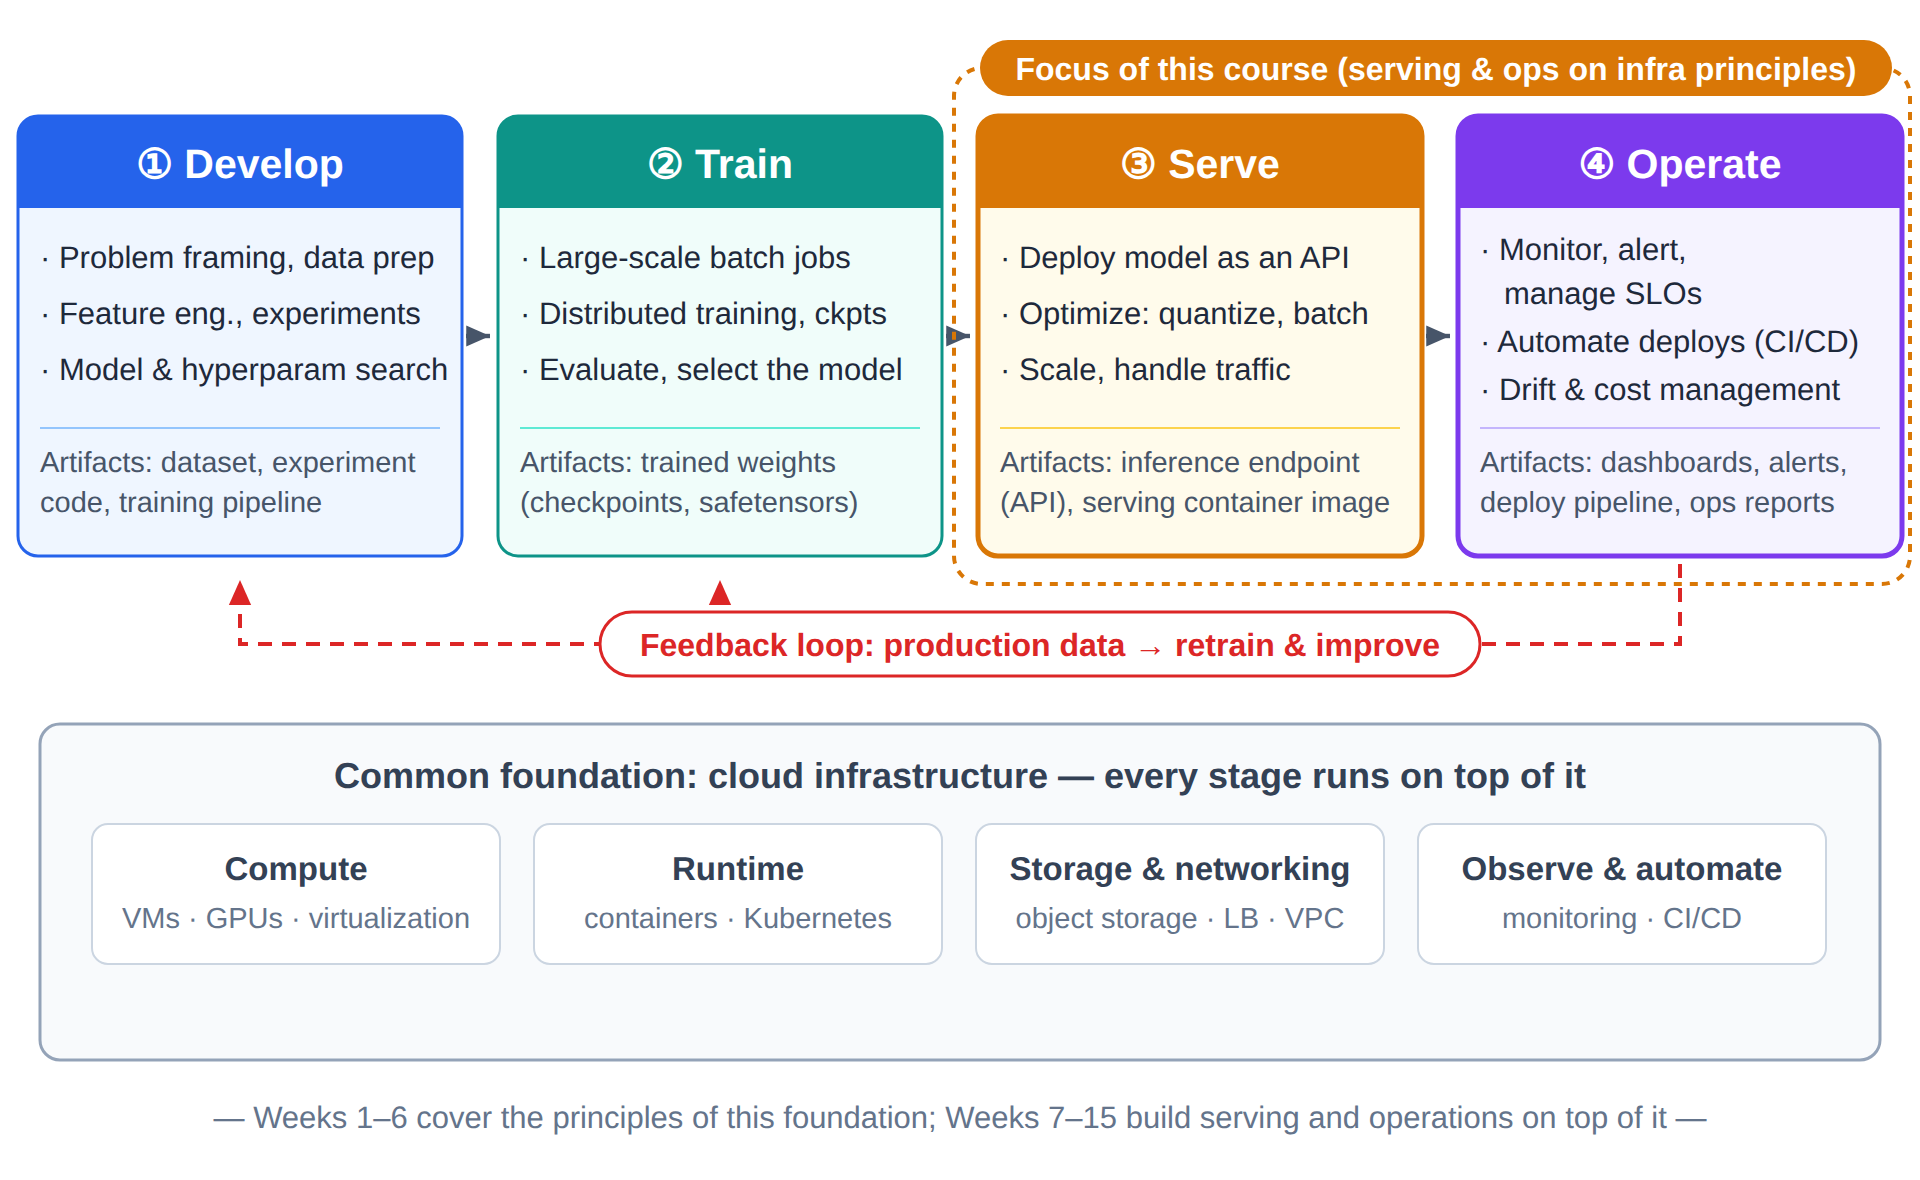
\includegraphics{figures/fig1-1_stack.png}}\\[3pt]
  \figcaption{그림 1-1  전체 AI 서비스 스택. 네 단계는 직선이 아니라 피드백으로 연결된 순환 고리를 이루며, 모든 단계가 클라우드 인프라 위에서 실행된다.}
\end{tbbfigure}

\subsection*{네 단계를 빠르게 둘러보기}

\textbf{① 개발} 단계에서는 문제를 정의하고, 데이터를 수집·정제하며, 모델 아키텍처와 학습 레시피를 실험한다. 주로 Jupyter 노트북과 실험 추적기를 사용한다. 인프라 관점에서 보면 작은 GPU를 짧고 빈번하게 사용하는 대화형 패턴이다. 이 단계의 산출물은 정제된 데이터셋과 재현 가능한 학습 파이프라인이다.

\textbf{② 학습} 단계에서는 그 파이프라인을 실제로 실행한다. 대형 모델의 경우 수십 개에서 수천 개 GPU에 걸친 분산 학습이 며칠 동안 이어지며, 장애에 대비해 중간중간 체크포인트를 저장한다. 이 단계의 산출물이자 이 책의 출발점은 \textbf{학습된 모델 가중치}다. 실제로는 체크포인트나 \code{safetensors} 같은 형식으로, 몇 기가바이트에서 수백 기가바이트에 이르는 파일이다. 모델 형식은 7주 차에 다룬다.

\textbf{③ 서빙} 단계에서는 모델 파일이 실제 트래픽을 처리하는 서비스가 된다. 모델을 추론 서버와 컨테이너로 감싸 클라우드에 배포하고 엔드포인트로 공개한다. 양자화와 배칭 같은 최적화로 지연 시간과 비용을 관리하며, 트래픽 변화에 맞춰 인스턴스 수를 조절한다. 이 책의 중반부 전체(7\textasciitilde{}12주 차)가 이 단계에 해당한다. 사례 A의 팀에 도움이 필요했던 곳도 바로 여기다.

\textbf{④ 운영} 단계는 서비스가 살아 있는 한 끝나지 않는다. 지연 시간, 처리량, 오류율, GPU 사용률을 계속 관찰하고, 새 모델 버전을 안전하게 배포하는 자동화 파이프라인을 구축한다. 또한 입력 분포가 모델의 학습 분포에서 벗어날 때 조용히 성능이 저하되는 \textbf{드리프트}를 감시한다. 13\textasciitilde{}15주 차의 주제다.

중요한 점은 이 네 단계가 \textbf{폭포형태가 아니라 순환고리(cycle)형태}라는 사실이다. 운영 과정에서 수집한 사용자 데이터와 실패 사례가 다시 개발과 학습으로 흘러 들어가 다음 모델 버전을 만들고, 새 모델은 다시 서빙 단계를 거친다. 조직이 성숙할수록 이 고리는 더 자동화되고 더 빠르게 돈다. 이 고리를 원활하게 돌리는 문화와 도구를 \textbf{MLOps}라 하며, 13주 차에 다룬다.

\subsection*{서빙 단계 확대하기}

이 책의 중심인 서빙 단계를 확대해 보자. 그림 1-2는 사용자 요청 하나가 도착해 응답으로 돌아오기까지의 경로를 추적한다. 요청은 먼저 API 게이트웨이(API gateway)와 로드 밸런서를 통과한다. 사례 A에서 뒤쪽 대기열이 인내 시간을 넘기자 504를 반환한 구성 요소가 바로 이들이다. 이곳에서 인증을 거친 요청은 여러 서빙 \textbf{레플리카} 중 하나로 전달된다. 레플리카 안에서 모델 실행은 전처리와 후처리 사이의 한 구간일 뿐이다. 모델 가중치는 시작할 때 \textbf{객체 스토리지(object storage) 기반 모델 저장소}에서 불러오며, 모니터링 시스템은 이 경로 곳곳에서 메트릭을 수집한다. 오토스케일러(autoscaler)는 이 근거를 이용해 레플리카 수를 조절한다.

\begin{tbbfigure}
  \adjustbox{max width=0.94\linewidth,max totalheight=0.46\textheight}{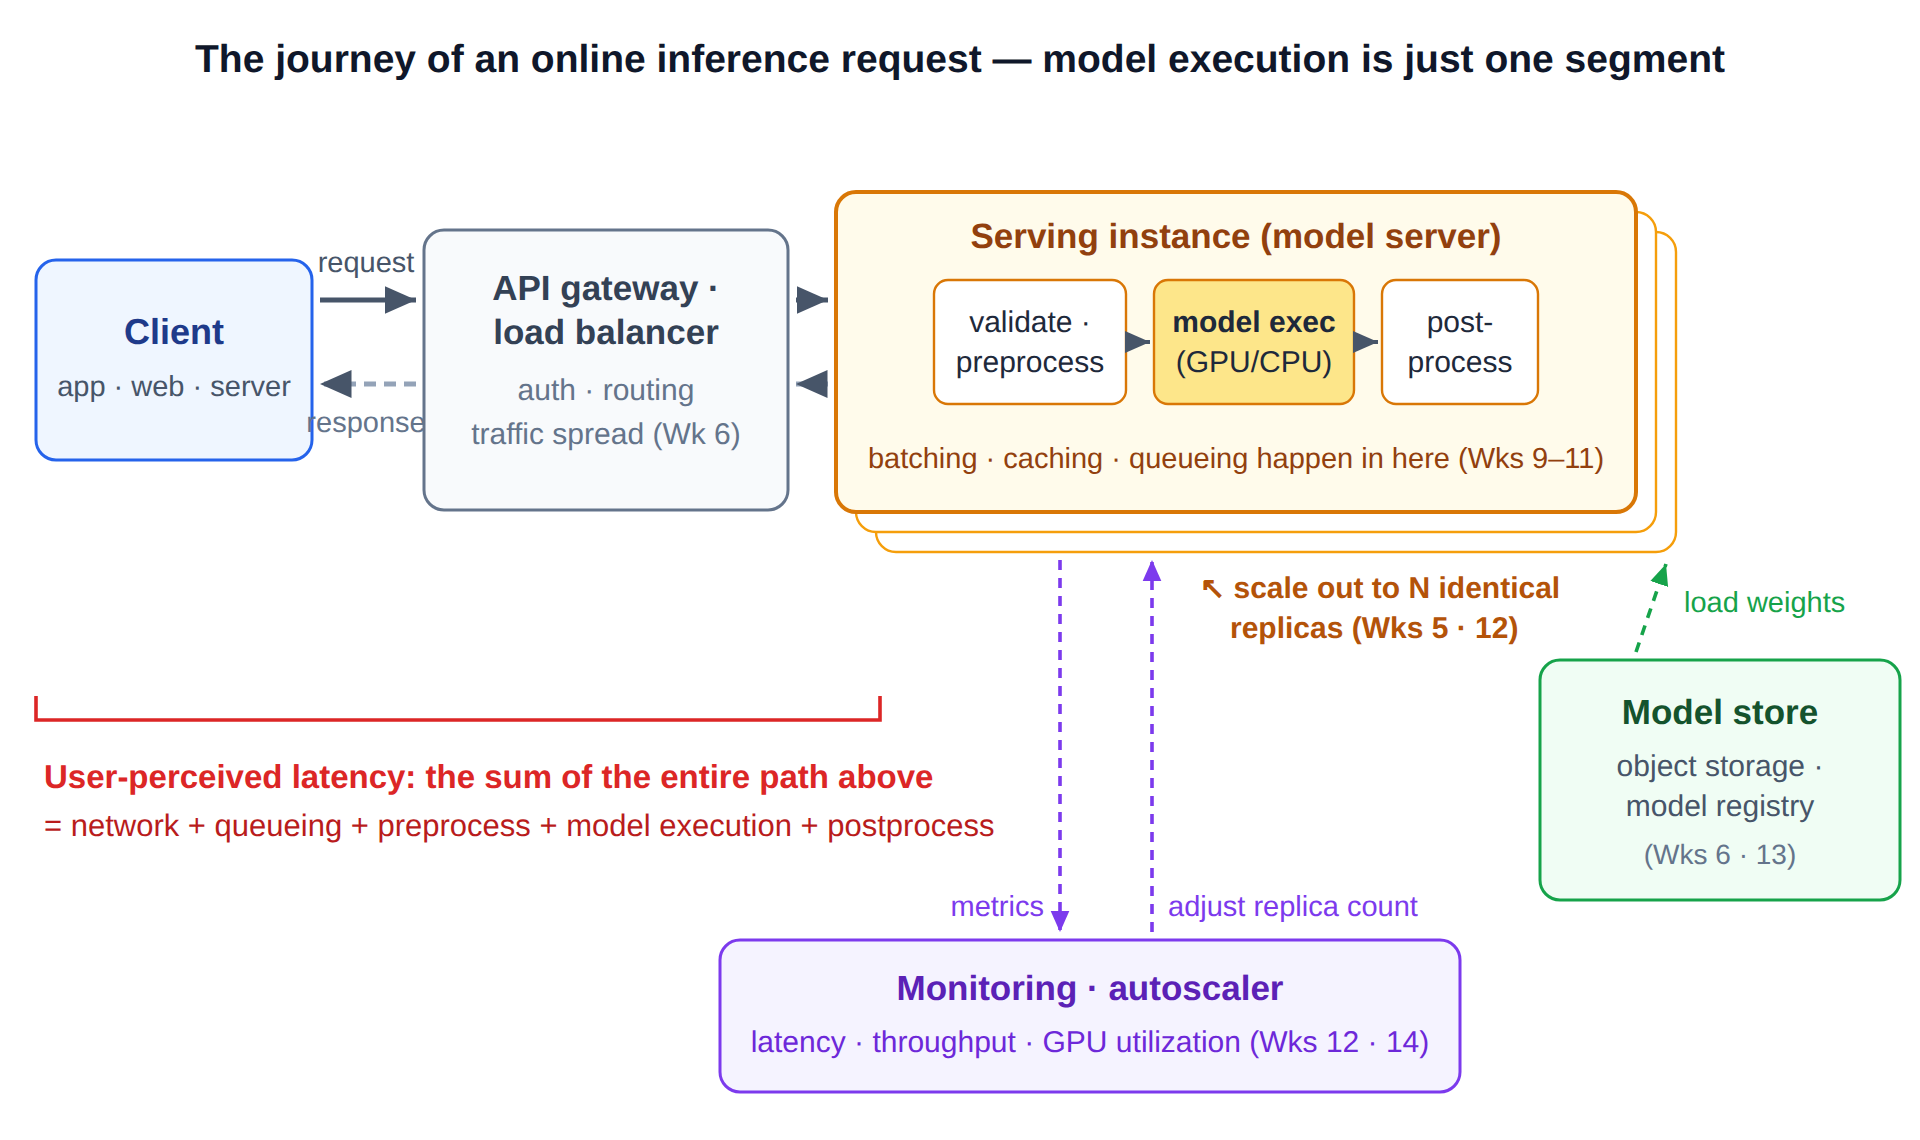
\includegraphics{figures/fig1-2_request_path.png}}\\[3pt]
  \figcaption{그림 1-2  온라인 추론 요청의 여정. 사용자가 체감하는 지연 시간은 모델 실행 시간이 아니라 전체 경로의 합이다.}
\end{tbbfigure}

이 그림에서 두 가지는 반드시 기억해야 한다. 첫째, \textbf{사용자가 체감하는 지연 시간은 전체 경로의 합이다.} GPU에서 모델 실행이 50 ms밖에 걸리지 않아도 요청이 대기열에서 2초를 기다렸다면 사용자는 느린 서비스를 경험한 것이다. 다른 해석의 여지가 없다. 사례 A는 극단적인 예였다. 30초의 경험 가운데 모델 시간이 0.31 s에 불과했다. 따라서 서빙 시스템의 성능 분석은 언제나 "어느 구간이 병목인가?"라는 질문이다. 둘째, 그림의 모든 구성 요소가 이 책 어딘가에서 다시 등장한다. 로드 밸런서와 객체 스토리지는 6주 차, 서빙 레플리카 내부의 배칭은 9\textasciitilde{}11주 차, 오토스케일러는 12주 차, 모니터링은 14주 차에 다룬다. 그림 1-2를 이 책의 지도라고 생각해도 좋다.

\begin{calloutbox}{tbbpurple}{tbbpurplefill}
{\normalsize\bfseries\color{tbbpurple}생각해 보기}\par\vspace{3pt}
\begin{tbbitemize}
  \item 그림 1-2의 지연 시간 구간을 직접 제어할 수 있는 것과 대부분 제어할 수 없는 것으로 나누어 보자. (힌트: 사용자의 네트워크는 누가 제어하는가?)
  \item 모델 가중치를 컨테이너 이미지에 넣지 않고 객체 스토리지에서 불러오는 이유는 무엇인가? 모델이 50 GB라면 어떤 문제가 생기는가? (6주 차에 답을 확인한다.)
\end{tbbitemize}
\end{calloutbox}

\section{학습 워크로드와 추론 워크로드}

같은 GPU와 같은 모델을 사용하더라도 인프라 관점에서 "학습"과 "추론 서빙"은 완전히 다른 존재다. 이 차이를 정확히 이해하는 것이 이 장의 가장 중요한 목표다. 서빙에서 작은 인스턴스를 여러 개 두어 수평확장(horizontal scale-out)하는 이유, 오토스케일링(autoscaling)이 필수인 이유, GPU 사용률이 골칫거리인 이유 등 이 책 전반에 등장하는 설계 결정이 모두 여기서 비롯되기 때문이다. 그림 1-3은 여섯 가지 관점에서 둘의 차이를 펼쳐 보인다.

\begin{tbbfigure}
  \adjustbox{max width=0.94\linewidth,max totalheight=0.46\textheight}{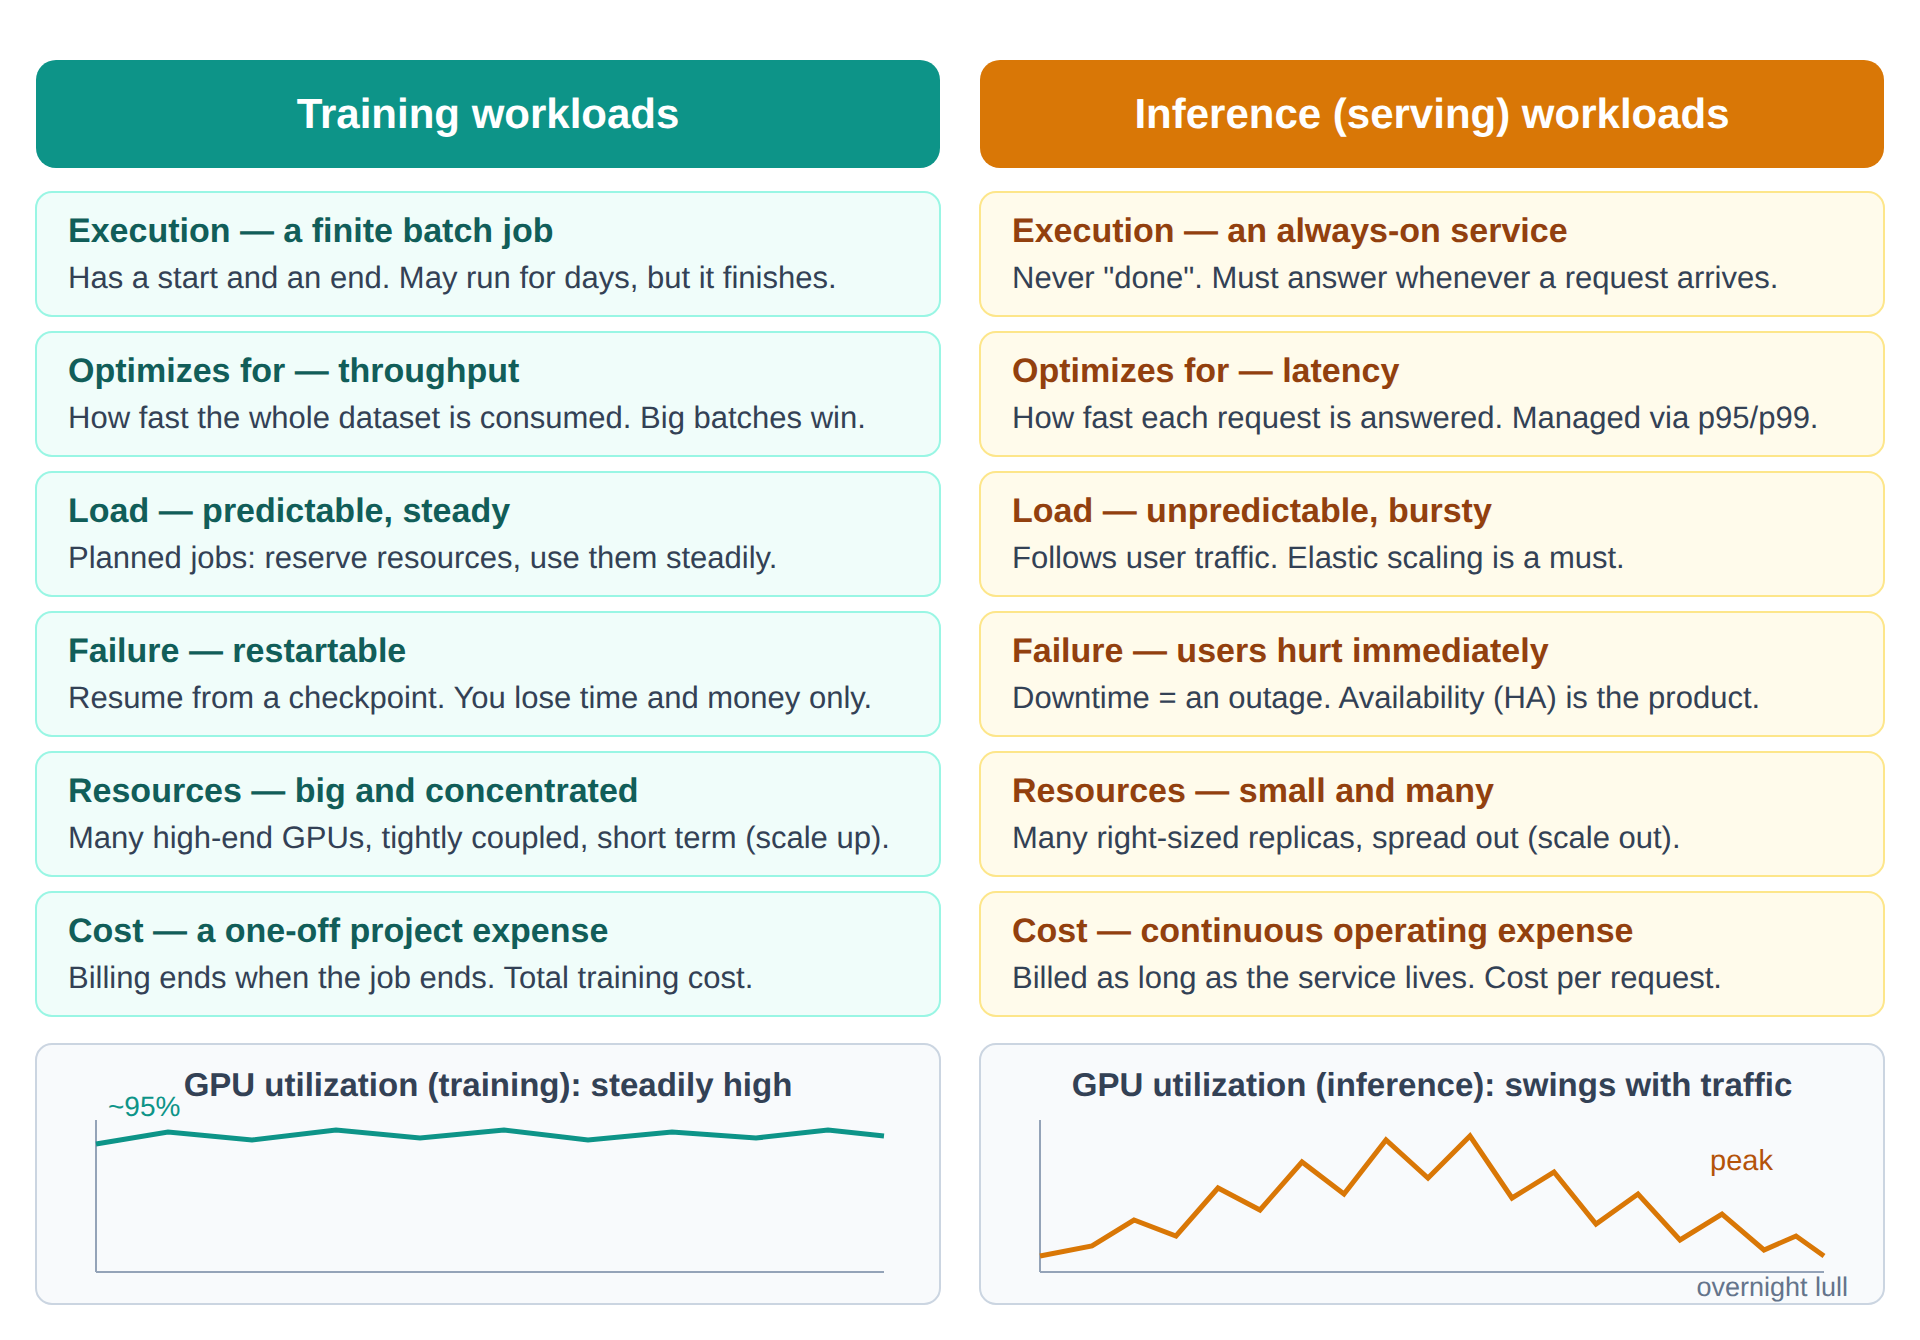
\includegraphics{figures/fig1-3_train_vs_infer.png}}\\[3pt]
  \figcaption{그림 1-3  학습 워크로드와 추론 워크로드. 아래쪽의 GPU 사용률 대비는 이 책 후반의 오토스케일링과 GPU 공유 주제를 예고한다.}
\end{tbbfigure}

\subsection*{작업과 서비스}

가장 근본적인 차이는 실행 형태다. 학습은 \textbf{시작과 끝이 있는 배치 작업}이다. 3일이 걸리든 3주가 걸리든, 끝나면 자원을 반납한다. 서빙은 \textbf{끝없이 상시 실행되는 서비스}다. 언제 도착할지 모르는 요청에 늘 응답할 준비가 되어 있어야 한다. 이 차이가 인프라를 바꾼다. 학습 플랫폼의 핵심 구성 요소는 작업 대기열과 배치 스케줄러다. 반면 서빙 플랫폼의 핵심은 로드 밸런서, 서비스가 계속 실행되도록 보장하는 오케스트레이터(Kubernetes Deployment가 하는 일이며 5주 차에 다룬다), 장애 자동 복구다. 사례 B가 벌어진 이유도 여기에 있다. \textit{작업}은 끝나면 머신을 반납하지만, \textit{서비스}에는 끝이 없으므로 머신을 기본적으로 끄는 스위치도 없다.

\subsection*{처리량 중심과 지연 시간 중심}

학습의 성능 지표는 처리량이다. 에포크(epoch)당 몇 시간이 걸리는지, 초당 몇 개 샘플을 처리하는지를 본다. 전체 실행이 더 일찍 끝난다면 개별 샘플에 0.1 s가 걸리는지 1 s가 걸리는지는 중요하지 않다. 따라서 학습은 GPU가 한 번에 처리하는 샘플 묶음인 \textbf{배치}를 \textbf{가능한 한 크게} 만들어 하드웨어를 포화시킨다.

서빙에서는 성능지표가 요청별 지연 시간으로 바뀌면서 근본적인 고민이 생긴다. GPU 관점에서는 요청을 더 큰 배치로 모을수록 처리량이 올라가고 비용이 낮아진다. 그러나 먼저 도착한 요청은 배치가 찰 때까지 \textbf{기다려야} 하므로 지연 시간이 나빠진다. 이 줄다리기는 서빙 시스템 설계 전체를 관통한다. 이를 영리하게 해결하는 동적 배칭(10주 차)과 연속 배칭(11주 차)은 이 책의 핵심 내용이다.

한 가지 더 기억하자. 서빙의 지연 시간은 평균이 아니라 \textbf{꼬리(tail)}로 관리한다. 평균 응답 시간이 100 ms여도 사용자 100명 중 한 명이 5초를 기다린다면, 하루 요청 100,000건을 처리하는 서비스는 매일 1,000번의 나쁜 경험을 제공한다. 따라서 실무에서는 모든 요청을 빠른 순서부터 느린 순서로 늘어놓았을 때 95번째와 99번째 백분위에 해당하는 지연 시간인 p95와 p99를 목표로 삼는다. "p99 ≤ 500 ms"는 요청의 99\%에 0.5초 안에 응답하겠다는 약속이다. 사례 A의 p99는 30초였으며, 모델이 아니라 대기열이 결정했다. 서비스 품질이 평균이 아니라 꼬리에 존재하는 이유가 바로 이것이다. 7주 차에는 이를 SLO로 발전시킨다.

\subsection*{서빙 삼각형: 지연 시간, 처리량, 비용}

배칭의 줄다리기는 이 책의 중심을 이루는 패턴의 한 사례이며, 별도의 이름과 그림을 붙일 만하다. 모든 서빙 시스템에는 세 가지가 요구된다. \textbf{낮은 지연 시간}(각 사용자에게 빠르게 응답), \textbf{높은 처리량}(초당 많은 사용자에게 응답), \textbf{낮은 비용}(응답 한 번에 적은 비용)이다. 엔지니어링의 현실은 \textit{어느 하나를 지불하면 나머지 둘을 살 수 있지만}, 어떤 묘수로도 셋을 한꺼번에 얻을 수는 없다는 것이다. 그림 1-7은 이 책의 나침반이다.

\begin{tbbfigure}
  \adjustbox{max width=0.94\linewidth,max totalheight=0.46\textheight}{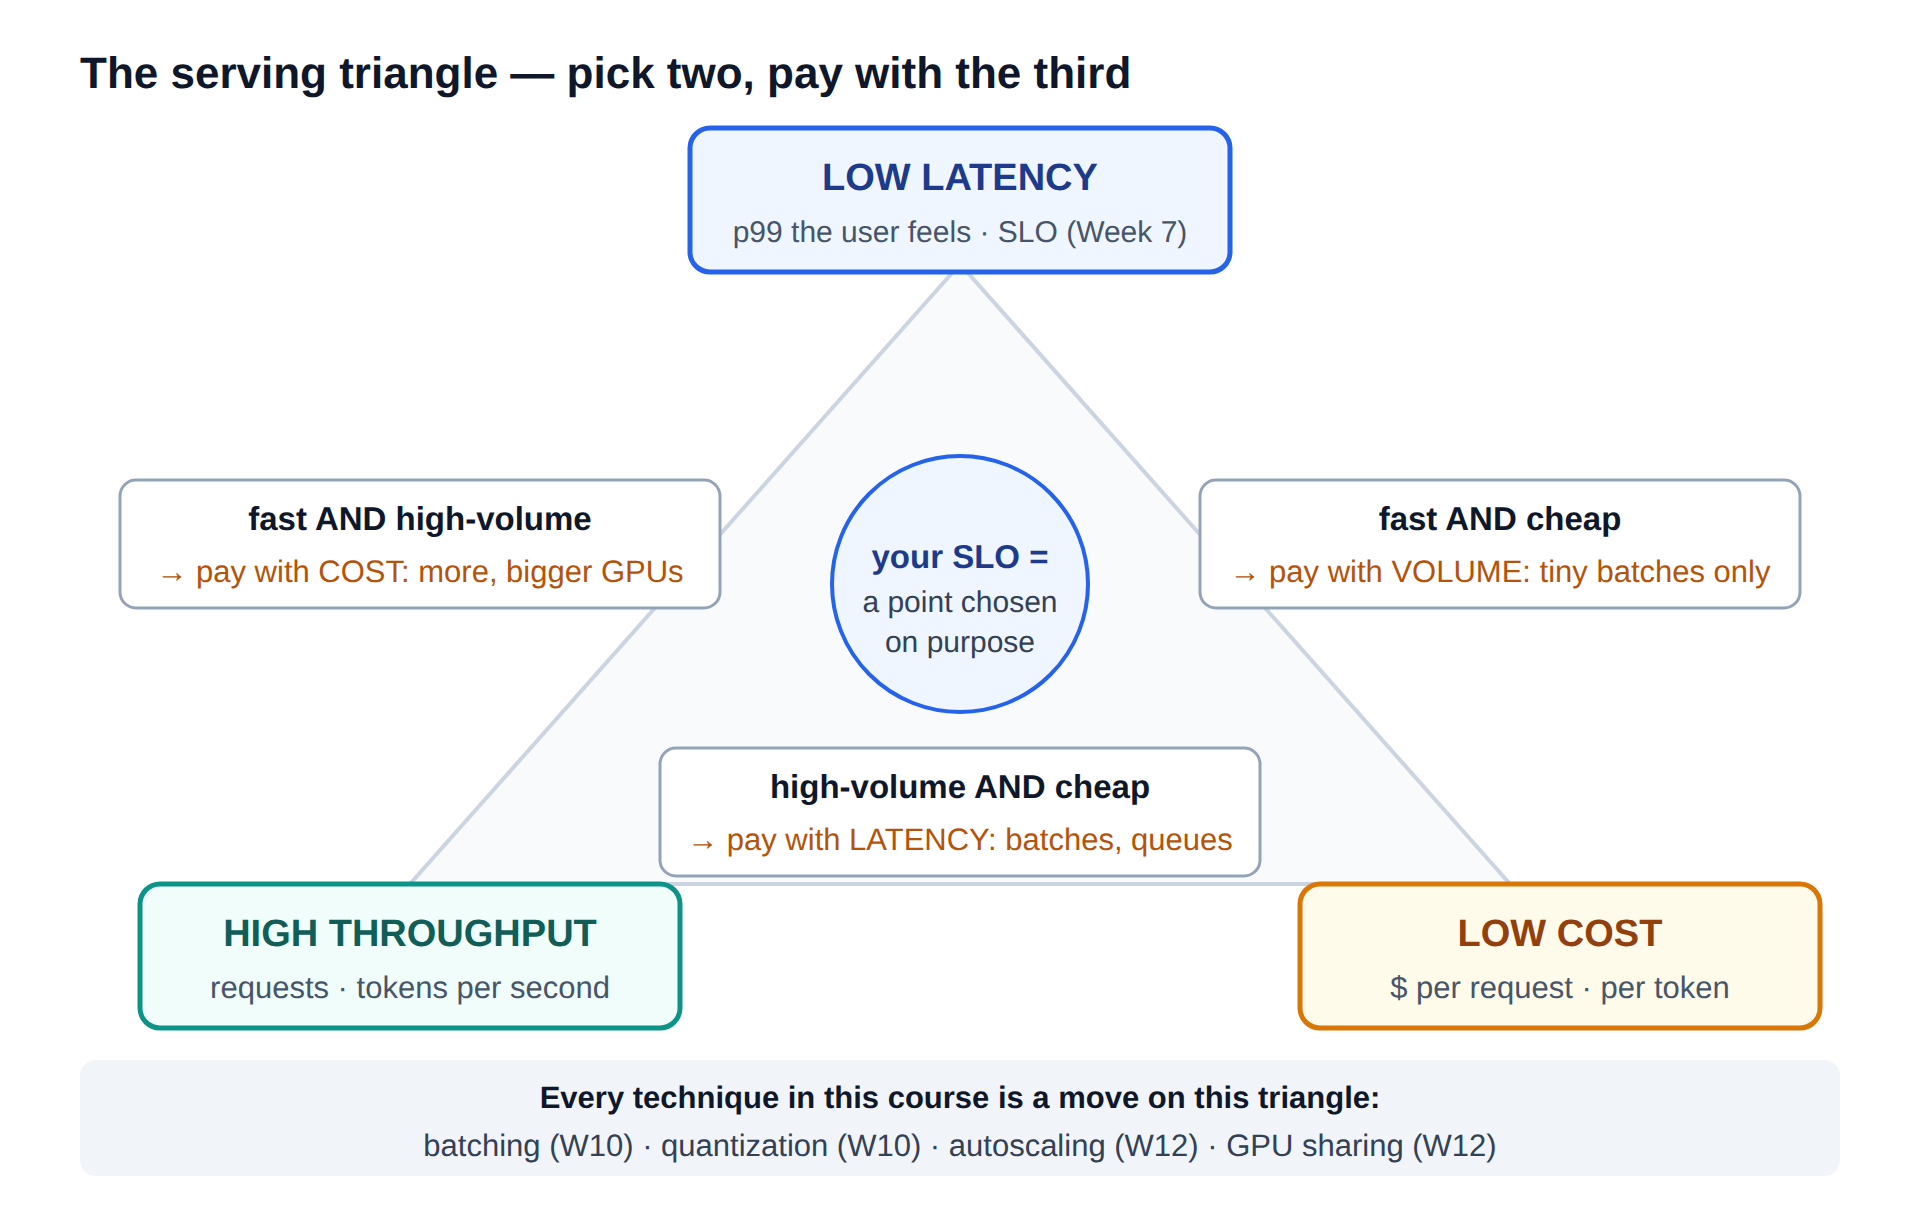
\includegraphics{figures/fig1-7_triangle.png}}\\[3pt]
  \figcaption{그림 1-7  서빙 삼각형. 이 책의 모든 최적화 기법은 이 삼각형 위에서 움직이는 일이며, 얻을 것을 취하기 전에 무엇을 지불하는지 밝히는 태도가 중요하다.}
\end{tbbfigure}

세 변을 한 바퀴 돌아보자. \textbf{빠르면서 대용량}인 서비스는 쉽게 만들 수 있다. 레플리카를 많이 실행하고 배치는 작게 유지하며 모든 곳에 여유 용량을 둔다. 대신 \textbf{비용}을 치른다(사례 B는 이 꼭짓점의 경고담이다. 아무도 쓰지 않는 용량이었다). \textbf{대용량이면서 저렴한} 서비스도 쉽다. 공격적으로 배칭하고 모든 GPU를 포화 상태에 가깝게 실행한다. 대신 \textbf{지연 시간}을 치른다. 파이프가 가득 차면 대기열이 생기고, 대기열은 꼬리에 자리하기 때문이다(사례 A가 의도치 않게 이 경우였다). \textbf{빠르면서 저렴한} 서비스도 트래픽이 늘기 전까지는 가능하다. 작고 준비된 인스턴스 하나가 적은 요청에 즉시 저렴하게 응답하다가 트래픽이 증가하는 순간 무너진다. 주어진 엔지니어링 역량으로 세 꼭짓점을 동시에 얻는 선택지는 \textit{없다}. 이 책이 가르치는 바를 한 문장으로 표현하면 \textbf{삼각형 자체를 바꾸는 방법}이다. 양자화(10주 차)는 요청 하나를 더 저렴하면서도 \textit{더} 빠르게 만들고, 연속 배칭(11주 차)은 단순 배칭보다 적은 지연 시간 비용으로 처리량을 얻으며, 오토스케일링(12주 차)은 트래픽이 많을 때만 비용의 꼭짓점으로 잠시 위치하게 한다.

이 삼각형에서 두 가지 규칙이 따라 나오며, 반드시 지켜야 한다. 첫째, \textbf{SLO는 바람이 아니라 선택한 점}이다. "200 req/s에서 p99 ≤ 500 ms, 월 \$900 이하"는 삼각형 안의 한 지점을 구체적으로 지목하고 지키겠다고 약속한다. 팀 프로젝트 제안서(7주 차)에서 바로 이 작업을 하며, 15주 차 시연은 그 약속을 기준으로 측정한다. 둘째, \textbf{모든 최적화 주장은 대가를 밝혀야 한다.} "더 빠르게 만들었다"는 말은 "GPU-hours가 X\% 늘어나는 대가로" 또는 "8보다 큰 배치 크기를 포기하여" 같은 설명이 뒤따라야 비로소 엔지니어링이 된다. 뒤 장에서 \textit{제1장의 비용 관점으로 읽으라}고 할 때 말하는 관점이 바로 이것이다. 어느 꼭짓점을 사기 위해 어느 꼭짓점으로 값을 지불하며, 그 교환은 그만한 가치가 있는가?

\subsection*{일정한 부하와 급증하는 부하}

학습 작업의 부하는 예측할 수 있다. 직접 시작한 작업이 직접 선택한 배치 크기로 실행된다. 서빙 워크로드의 부하는 사용자가 결정한다. 점심시간에 급증하고 밤에는 조용해지며, 마케팅 행사나 입소문을 탄 게시물 때문에 10배로 뛸 수도 있다. 사례 A의 Discord 메시지는 소규모 바이럴 게시물이었고, ChatGPT 출시는 그 완전한 규모의 사례였다. 이 특성은 서빙 인프라의 고전적인 딜레마를 만든다. \textbf{최대치에 맞춰 프로비저닝하면 한산할 때 돈을 낭비하고}(트래픽이 10분의 1인 오전 4시에도 GPU 10개가 돌아간다. 서버군 규모의 사례 B다), \textbf{평균에 맞춰 프로비저닝하면 최대치에서 서비스가 무너진다}(사례 A). 해결책은 부하에 맞춰 자원을 늘리고 줄이는 오토스케일링이며, 논리적 극단에는 요청이 없을 때 인스턴스를 0개로 만드는 0으로 스케일링(scale-to-zero)이 있다. 그러나 GPU 서빙 인스턴스가 준비되려면 수십 초에서 몇 분이 걸린다. 모델 로딩이 느린 부분이다. 이것이 \textbf{콜드 스타트(cold start)} 문제이며, 12주 차에 이 문제를 만날 때 2주 차의 Firecracker microVM에서 해결책을 찾는다.

\subsection*{장애가 지니는 무게}

학습 중 GPU가 죽으면 성가시지만 재앙은 아니다. 마지막 체크포인트부터 재개하면 된다. 잃는 것은 시간과 돈이다. 서빙 장애는 성격부터 다르다. \textbf{바로 지금 서비스를 사용하는 사람들이 즉시 피해를 본다.} 오류 페이지를 보거나 로딩 표시만 바라보다 떠난다. 따라서 서빙 시스템은 단일 장애점(single point of failure)을 없애는 데 집착한다. 항상 레플리카를 둘 이상 실행하고, 죽은 인스턴스를 자동으로 교체하며(Kubernetes의 자가 치유, 5주 차), 새 버전 출시 때는 트래픽의 작은 비율만 새 버전에서 처리하기 시작하여 점진적으로 새 버전으로 모두 이전한다(카나리 배포, 13주 차).

\subsection*{자원 사용의 형태 — 시간에 따른 형태까지}

메모리 요구량은 근본부터 다르다. 학습은 가중치뿐 아니라 그래디언트, 옵티마이저 상태(Adam에서는 가중치의 두 배), 중간 활성값(activations)까지 GPU 메모리에 보관해야 한다. 추론에는 가중치와 현재 요청의 활성값만 필요하다. 경험칙상 같은 모델에서 추론에 필요한 메모리는 학습의 약 3분의 1에서 4분의 1이다. 가중치의 수치 정밀도를 낮추는 \textbf{양자화}(10주 차)를 적용하면 더 줄어든다. 따라서 최신 대형 GPU가 없어도 추론을 실행할 수 있으며, 이 책의 실습도 T4 한 대나 Colab 세션 하나에 맞도록 설계했다.

그러나 "메모리를 덜 쓴다"를 "메모리 사용량이 일정하다"로 받아들이면 안 된다. 추론 서버의 메모리 사용량에는 \textbf{시간에 따른 형태}가 있고, 그 형태는 뾰족하게 출렁인다. 가중치는 한 번 로드되어 계속 상주하는 평평한 기준선이다. 그 위에 처리 중인 요청마다 활성값용 작업 메모리를 할당하며, 이 할당량은 \textbf{동시에 처리하는 요청 수(배치)와 각 입력의 크기}에 비례한다(LLM에서는 시퀀스 길이와 요청마다 커지는 KV 캐시라는 구조가 중요하며, 11주 차의 주인공이다). 유휴 상태에서 6 GB를 쓰는 서버도 긴 입력이 한꺼번에 몰리는 순간 8 GB를 훌쩍 넘길 수 있다. 사례 A를 떠올려 보자. 프로덕션 트래픽은 바로 이렇게 급증한다. 따라서 \textit{서버를 하루 동안 유휴 상태로 관찰하고 10\%를 더한 값을 메모리 한도로 설정한다}는 흔히 쓰는 용량 산정 규칙은 신중함이 아니라 예정된 장애다. 이 한도는 조용한 모든 시간에는 유지되다가 처음으로 실제 요청이 몰리는 순간 서버를 다운시키고 로그에 \code{137}을 남긴다(요청당 몇 킬로바이트의 문자열만 사용하는 많은 무상태(stateless) 웹 앱에는 같은 규칙이 잘 통한다. 그래서 이런 습관이 생겼고, 추론에 적용하면 위험한 이유도 여기에 있다). 3주 차에는 이 서버다운 메커니즘의 실제 이름인 cgroup과 OOM 킬러를 배운다.

하드웨어 선택도 갈린다. 학습은 그래디언트 동기화로 통신량이 많으므로 NVLink와 InfiniBand로 긴밀하게 연결한 고성능 GPU(H100, B200급) 클러스터를 선호한다. 추론 레플리카끼리는 거의 통신하지 않으므로 저렴한 추론 GPU(L4, T4)를 여러 곳에 분산하는 편이 보통 더 싸다. 소형 모델은 \code{llama.cpp} 같은 런타임으로 CPU에서도 서빙할 수 있으며, GPU가 없을 때 사용하는 대안이기도 하다.

\begin{calloutbox}{tbbteal}{tbbtealfill}
{\normalsize\bfseries\color{tbbx115E59}상자 1-1  GPU를 사용하는 이유 — 유휴 GPU가 문제인 이유}\par\vspace{3pt}
딥러닝 계산의 본질은 거대한 행렬 곱셈이며, 행렬 곱셈은 동시에 실행할 수 있는 수천 개의 작고 독립적인 계산으로 나뉜다. GPU는 수천 개 코어로 정확히 이 작업을 수행하도록 만든 하드웨어다. CPU가 뛰어난 일꾼 몇 명이라면, GPU는 단순한 일꾼 수천 명으로 이루어진 여단이다.

문제는 가격이다. 데이터 센터 GPU 서버는 시간당 몇 달러가 든다(1.5절). 학습은 GPU를 95\% 이상 바쁘게 유지한 뒤 반납하지만, 사용자 트래픽을 따르는 추론 서비스는 평균 사용률이 흔히 수십 퍼센트 이하로 떨어진다. 사례 B의 0.2\%는 정도가 극단적일 뿐이다. \textbf{비싼 자원이 놀고 있는 상태}가 AI 서빙 비용 문제의 본질이며, 배칭(10주 차), GPU 공유와 MIG(2·12주 차), 오토스케일링(12주 차), 스팟 인스턴스(12주 차)는 모두 이 문제를 공략한다.
\end{calloutbox}

\vspace{3.0pt}

\subsection*{비용의 형태: 일회성 지출과 지속적 지출}

마지막은 비용 구조다. 학습 비용은 프로젝트 형태다. "이번 학습 실행에 400 GPU-hours, 약 X달러가 들었다"처럼 한 번 지불하면 끝난다. 서빙 비용은 \textbf{서비스가 살아 있는 동안 매달 반복되는 운영 비용}이다. 트래픽과 함께 늘어나며, 방치하면 조용히 부풀어 오른다. 따라서 서빙 비용은 총액이 아니라 \textbf{요청당 비용}(또는 토큰당 비용)으로 관리한다. 이 지표는 최적화의 성공 기준(10주 차)이자 팀 프로젝트의 필수 산출물인 월간 운영 비용 추정치다.

요청당 비용 계산에서 따라오는 한 가지 결과는 별도의 문장으로 강조할 만하다. 제5장이 이 개념에 크게 의존하기 때문이다. 청구서는 머신 단위로 오지만 가치는 요청 단위로 생기므로, 서빙 경제성은 \textbf{밀도}라는 게임을 끊임없이 한다. 서로 해치지 않으면서 머신 한 대를 레플리카 몇 개가 공유할 수 있는가? 각 레플리카에 넉넉한 전용 여유 용량을 주면 머신당 실행하는 레플리카 수가 적어진다. 안전하지만 비싸다. 촘촘히 넣으면 레플리카 하나의 부하 급증이 이웃 레플리카의 지연 시간 급증으로 이어진다. 따라서 레플리카당 여유 용량 1 GB는 모두 \textbf{의도적으로 선택한 밀도와 비용의 절충}이다. 자원 요청량과 한도라는 도구를 이용하면 이 절충을 강제할 수 있으며, 제3장과 제5장이 바로 이를 향해 나아간다.

정리하면, 이 책 후반부의 모든 주제는 이 절에서 살펴본 대비의 귀결이다. 서빙은 상시 실행 서비스이므로 오케스트레이션(orchestration)과 자가 치유(self-healing)가 필요하고(5주 차), 지연 시간 중심이므로 배칭과 최적화가 어렵고도 흥미로우며(10\textasciitilde{}11주 차), 부하가 급증하므로 오토스케일링과 콜드 스타트가 중요하고(12주 차), 장애의 무게가 크므로 배포 전략과 모니터링이 정교해야 한다(13\textasciitilde{}14주 차). 이 문장과 삼각형을 이 장의 요약으로 기억해 두자.

\begin{calloutbox}{tbbpurple}{tbbpurplefill}
{\normalsize\bfseries\color{tbbpurple}생각해 보기}\par\vspace{3pt}
\begin{tbbitemize}
  \item 온라인 상점의 상품 추천 모델을 생각해 보자. 이 모델의 "학습"과 "서빙"에 대해 그림 1-3의 여섯 차원별로 구체적인 수치를 그려 보자. (예를 들어 최대 트래픽은 언제인가?)
  \item 무료 취미 프로젝트, 주식 거래 신호 API, 사진 보관소를 밤새 처리하는 배치 캡셔너를 서빙 삼각형(serving triangle) 위에 배치해 보자. 각 서비스는 어느 꼭짓점을 희생하며, 어떤 SLO 수치를 적을 것인가?
  \item 어떤 추론은 실시간일 필요가 없다. 예를 들어 어제 찍은 사진을 밤새 분류할 수 있다. 이런 "배치 추론"은 그림 1-3의 어느 열과 닮았는가? 인프라에서 무엇이 단순해지는가? (7주 차 예고.)
\end{tbbitemize}
\end{calloutbox}

\section{클라우드 서비스 모델과 AI 인프라}

앞 절에서 살펴본 추론 워크로드의 특성, 즉 급증하는 부하, 상시 운영, 비싼 GPU는 자연스럽게 한 가지 질문으로 이어진다. \textbf{이 인프라는 어디에 두어야 하며, 그중 얼마만큼을 직접 관리해야 하는가?} 사례 B의 팀은 반사적으로 "VM 하나를 빌려 모든 것을 직접 설치한다"고 답했고 그 대가로 \$779를 냈다. 이 절에서는 팀이 생각하지 못했던 선택지를 정리한다.

\subsection*{클라우드를 사용하는 이유}

GPU 서버를 직접 구매해 온프레미스에서 운영하는 방식과 비교하면, AI 워크로드에서 클라우드의 장점은 특히 두드러진다. 첫째, \textbf{자본 지출이 운영 지출로 바뀐다.} 데이터 센터급 GPU 서버는 수만에서 수십만 달러가 들지만, 클라우드에서는 시간당 몇 달러에 빌리고 작업이 끝나면 떠날 수 있다. 둘째는 \textbf{탄력성}이다. 임대한 인프라만이 1.3절에서 본 급증하는 추론 부하에 맞춰 늘고 줄 수 있다. 셋째, \textbf{하드웨어 세대교체의 위험을 이전한다.} 1\textasciitilde{}2년마다 새 GPU가 출시되고 구형 GPU의 가치는 빠르게 떨어지지만, 클라우드에서는 인스턴스 유형만 바꾸면 된다. 물론 클라우드가 항상 정답은 아니다. 대규모 자원을 계속 높은 사용률로 쓰는 조직은 결국 소유하는 편이 더 저렴하며, 어떤 데이터는 건물 밖으로 반출할 수 없다. 그러므로 정확한 질문은 "클라우드를 쓸 것인가?"가 아니라 "\textbf{어느 수준까지 빌릴 것인가?}"다.

\subsection*{고전적인 세 계층: IaaS, PaaS, SaaS}

전통적으로 클라우드 서비스는 공급자가 얼마나 많이 관리해 주는지에 따라 분류한다. \textbf{IaaS}(Infrastructure as a Service)는 가상 머신, 스토리지, 네트워크 같은 원재료를 빌려 주며, OS 위의 모든 것은 사용자의 책임이다. \textbf{PaaS}(Platform as a Service)는 런타임 플랫폼까지 관리하므로 애플리케이션만 가져오면 된다. \textbf{SaaS}(Software as a Service)는 완성된 소프트웨어를 그대로 사용하는 형태다. 아래로 갈수록 제어권이 많아지고, 위로 갈수록 운영할 대상이 줄어든다.

AI 인프라는 이 세 계층을 이어받으면서 그 사이에 더 세밀한 단계를 넣는다. 그림 1-4가 이 스펙트럼을 보여 준다.

\begin{tbbfigure}
  \adjustbox{max width=0.94\linewidth,max totalheight=0.46\textheight}{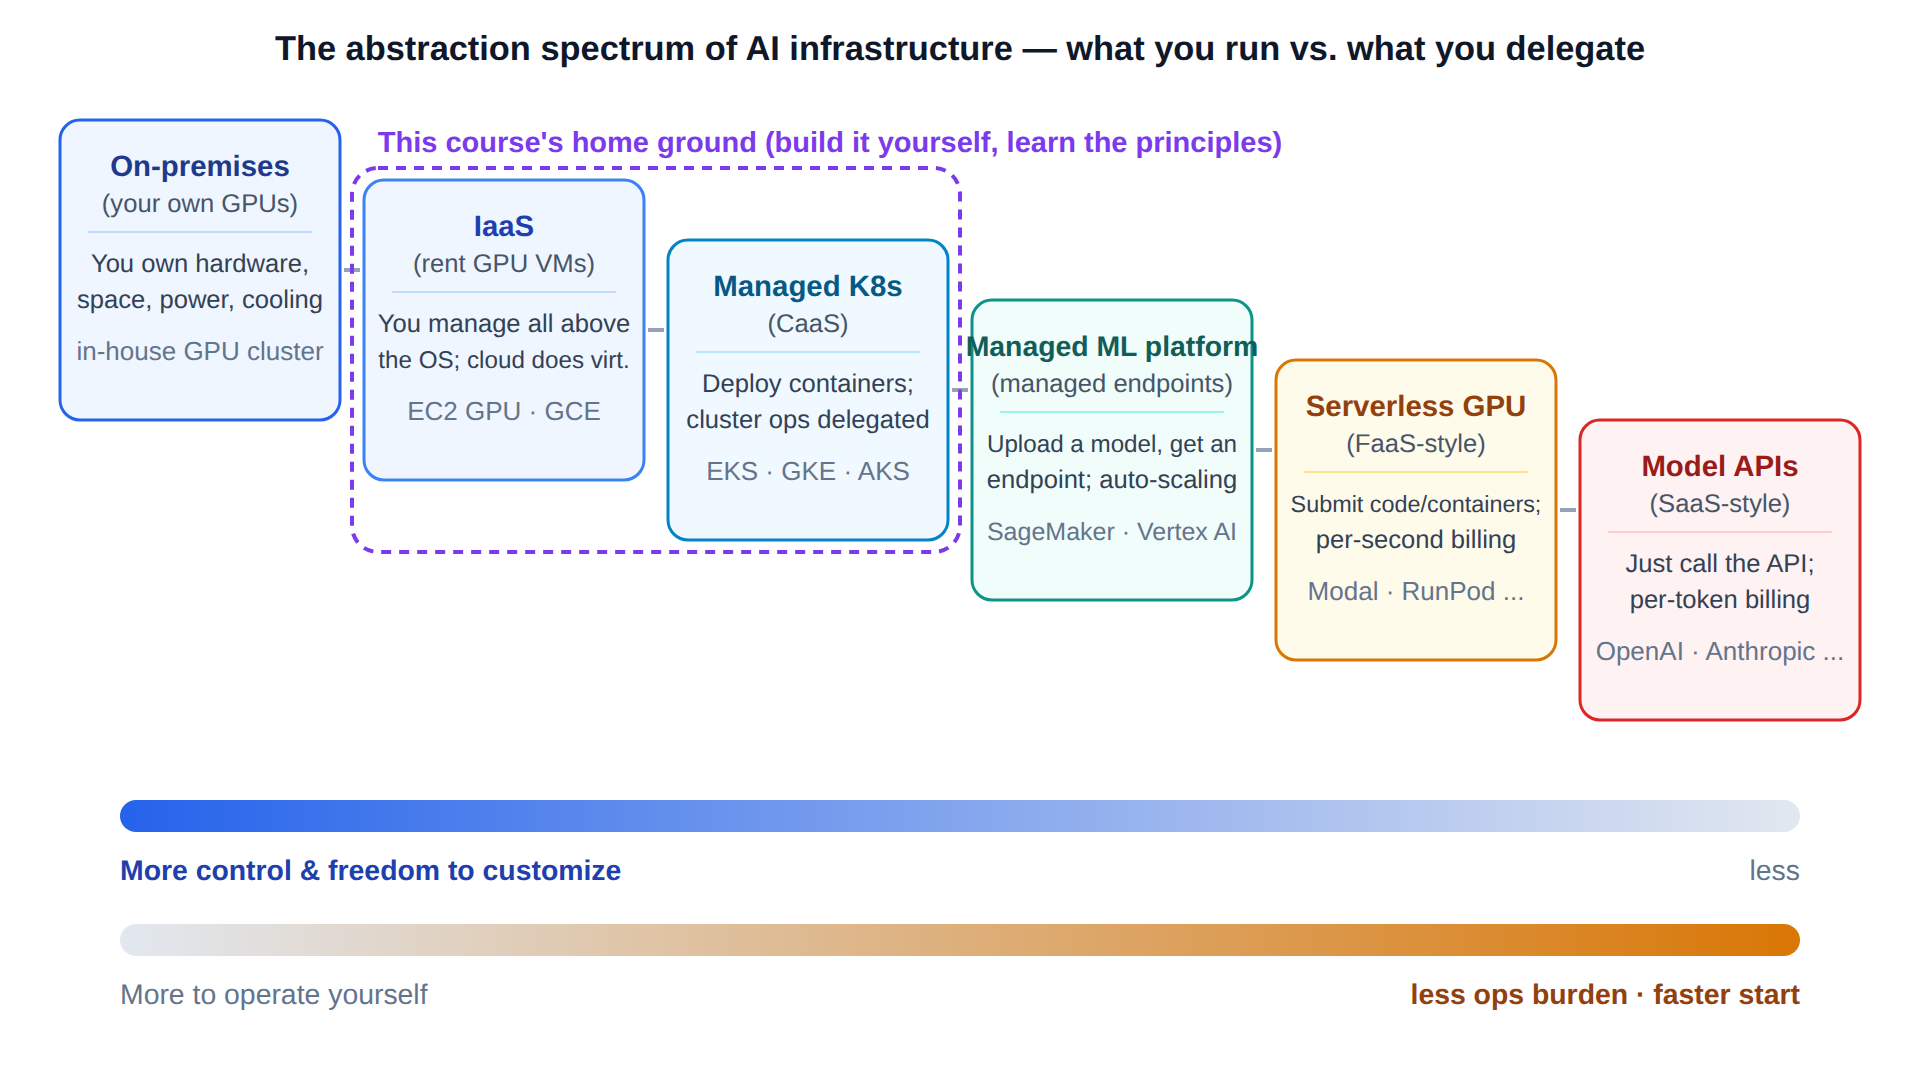
\includegraphics{figures/fig1-4_abstraction.png}}\\[3pt]
  \figcaption{그림 1-4  AI 인프라의 추상화 스펙트럼. 오른쪽으로 갈수록 운영할 대상이 줄지만 제어권도 줄어든다. 이 책은 의도적으로 IaaS부터 관리형 K8s까지의 범위를 다룬다.}
\end{tbbfigure}

각 단계를 서빙 관점에서 읽어 보자. \textbf{GPU VM (IaaS)}은 GPU가 장착된 머신 전체를 빌려 준다. 무엇이든 할 수 있지만 OS 패치부터 장애 복구까지 모든 일을 직접 해야 한다. \textbf{관리형 Kubernetes (CaaS)}는 컨테이너 오케스트레이션 클러스터를 빌려 준다. 컨테이너의 배포, 스케일링, 복구는 플랫폼이 처리한다. 오늘날 자체 관리형 서빙의 사실상 표준이며 이 책의 주 무대다(5주 차). \textbf{관리형 ML 플랫폼}(SageMaker, Vertex AI 등)은 "모델 파일을 건네면 엔드포인트를 받는" 수준까지 올라간다(13주 차에 소개한다). \textbf{서버리스 GPU} 플랫폼은 컨테이너나 함수만 받아 요청을 처리하는 동안에만 GPU를 할당하고 초 단위로 과금한다. 콜드 스타트(12주 차)를 감수하는 대신 사례 B가 수학적으로 일어날 수 없다. 가장 오른쪽의 \textbf{모델 API}는 다른 사람의 인프라에서 다른 사람의 모델을 사용하고 토큰 단위로 비용을 내는 방식, 즉 AI를 SaaS처럼 소비하는 형태다.

\begin{tbbtablewrap}
  \begin{tabular}{@{}>{\raggedright\arraybackslash}m{\dimexpr 0.2021\tbltextwidth-2\tabcolsep\relax} >{\raggedright\arraybackslash}m{\dimexpr 0.2660\tbltextwidth-2\tabcolsep\relax} >{\raggedright\arraybackslash}m{\dimexpr 0.2766\tbltextwidth-2\tabcolsep\relax} >{\raggedright\arraybackslash}m{\dimexpr 0.2553\tbltextwidth-2\tabcolsep\relax}@{}}
  \arrayrulecolor{tbbnavy}\specialrule{1pt}{0pt}{0pt}
  \rowcolor{tbbtablehead}{\centering \bfseries\color{tbbnavy}계층} & {\centering \bfseries\color{tbbnavy}빌리는 것} & {\centering \bfseries\color{tbbnavy}직접 관리할 것} & {\centering \bfseries\color{tbbnavy}서빙 예시} \\
  \arrayrulecolor{tbbnavy}\specialrule{0.7pt}{0pt}{2pt}
  {\textbf{IaaS}} & {GPU VM, 스토리지, 네트워크} & {OS, 런타임, 서빙 소프트웨어, 스케일링, 복구} & {EC2/GCE GPU 인스턴스에 vLLM을 직접 설치} \\
  \arrayrulecolor{tbbtableborder}\hline
  {\textbf{CaaS}} & {+ K8s 클러스터 운영} & {컨테이너 이미지, 배포 명세, 서빙 구성} & {EKS · GKE의 모델 서버(이 책)} \\
  \arrayrulecolor{tbbtableborder}\hline
  {\textbf{PaaS / ML 플랫폼}} & {+ 서빙 런타임, 스케일링, 배포} & {모델 아티팩트, 구성} & {SageMaker · Vertex AI 엔드포인트} \\
  \arrayrulecolor{tbbtableborder}\hline
  {\textbf{서버리스 GPU}} & {+ 전체 인스턴스 수명 주기} & {컨테이너/함수 코드} & {Modal, RunPod Serverless, ...} \\
  \arrayrulecolor{tbbtableborder}\hline
  {\textbf{SaaS (모델 API)}} & {모델과 인프라 전체} & {프롬프트, 호출 코드} & {OpenAI, Anthropic 등의 모델 API} \\
  \arrayrulecolor{tbbnavy}\specialrule{1pt}{2pt}{0pt}
  \end{tabular}\par
  \figcaption{표 1-2  서비스 계층별 서빙: 빌리는 것과 직접 관리하는 것}
\end{tbbtablewrap}

이 책이 택한 교육 방식도 분명히 해 두자. 업계에서는 표의 아래쪽 행, 즉 추상화 수준이 높은 선택지를 고르는 것이 합리적일 때가 많다. 그럼에도 이 책은 IaaS에서 CaaS까지의 길을 따라 \textbf{직접 구축한다}. 높은 추상화 수준에서 무언가 고장 났을 때 아래에서 어떤 일이 일어나는지 아는 사람과 모르는 사람은 전혀 다르게 대응하기 때문이다. 관리형 엔드포인트의 청구서를 해석하거나 서버리스 플랫폼의 콜드 스타트를 줄이는 일도 결국 아래 계층에 대한 이해를 요구한다. 처음부터 한 번 직접 만들어 보면 어떤 추상화도 다시는 두렵지 않을 것이다.

\begin{calloutbox}{tbbpurple}{tbbpurplefill}
{\normalsize\bfseries\color{tbbpurple}생각해 보기}\par\vspace{3pt}
\begin{tbbitemize}
  \item 수강 신청 기간에만 트래픽이 급증하는 교내 챗봇을 만든다고 하자. 그림 1-4에서 어느 지점을 선택하겠는가? 유휴 비용과 가용한 운영 인력을 근거로 논증해 보자.
  \item "공동 책임 모델(shared responsibility model)"이라는 표현을 찾아보자. 관리형 K8s에서 보안 사고가 발생하면 어느 부분이 공급자의 책임이고 어느 부분이 사용자의 책임인가?
\end{tbbitemize}
\end{calloutbox}

\section{GPUaaS와 모델 API 생태계}

이제 실제 시장을 살펴보자. 지난 몇 년 동안 두 극점 사이에서 생태계가 폭발적으로 성장했다. 하나는 GPU 계산 자원 자체를 판매하는 \textbf{GPUaaS}(GPU-as-a-Service), 다른 하나는 모델의 역량 자체를 판매하는 \textbf{모델 API}다. 시장은 빠르게 변하므로 이 절의 목표는 회사 이름을 외우는 것이 아니라 \textbf{지형을 읽는 법}을 익히는 데 있다.

\subsection*{하드웨어 감각: 데이터 센터 GPU}

시장보다 먼저 상품부터 살펴보자. NVIDIA는 데이터 센터 GPU의 사실상 표준이며, 세대가 바뀔 때마다 속도뿐 아니라 \textbf{메모리}도 커진다. A100 (40/80 GB) → H100 (80 GB) → H200 (141 GB) → Blackwell 세대 B200 (192 GB)로 이어지며, 여러 CPU와 GPU를 하나의 장치로 결합한 GB200 NVL72 같은 랙 규모 시스템도 있다. 서빙에서 메모리가 이토록 중요한 이유는 무엇인가? \textbf{추론을 실행하려면 모델이 GPU 메모리에 들어가야 하기} 때문이다. 16-bit 정밀도의 파라미터가 700억 개인 모델은 가중치만 약 140 GB가 필요하므로 80 GB H100 한 대에 들어가지 않는다. 양자화(10주 차)로 줄이거나 여러 GPU에 샤딩해야 한다. 한편 추론용 GPU인 L4 (24 GB), T4 (16 GB)는 저렴하고 전력 효율이 높은 일꾼이며, 이 책의 실습은 T4 한 대를 기준으로 설계했다.

여기서 이 책 내내 본능이 될 때까지 반복할 용량 산정 원칙이 처음 등장한다. \textbf{먼저 결정적인 제약 차원을 찾아라.} 대부분의 추론에서 실제 제약은 순수 FLOPs가 아니라 메모리 용량(모델이 들어가는가?)이나 메모리 대역폭(가중치가 계산 장치를 얼마나 빠르게 통과할 수 있는가?)이다. 그래서 소형 모델은 적당한 L4에서도 훨씬 저렴한 가격으로 H100과 거의 같은 사용자 경험을 제공할 때가 많다. "안전을 위해" 가장 큰 GPU를 고르는 일은 대개 애초에 제약이 아니었던 차원에 돈을 내는 셈이다. 인스턴스는 결정적인 제약 차원에 따라 선택해야 하며, 이후의 모든 비용 연습(9·10·12주 차)은 여기서 시작한다.

\begin{tbbtablewrap}
  \begin{tabular}{@{}>{\raggedright\arraybackslash}m{\dimexpr 0.3830\tbltextwidth-2\tabcolsep\relax} >{\raggedright\arraybackslash}m{\dimexpr 0.2553\tbltextwidth-2\tabcolsep\relax} >{\raggedright\arraybackslash}m{\dimexpr 0.3617\tbltextwidth-2\tabcolsep\relax}@{}}
  \arrayrulecolor{tbbnavy}\specialrule{1pt}{0pt}{0pt}
  \rowcolor{tbbtablehead}{\centering \bfseries\color{tbbnavy}임대처} & {\centering \bfseries\color{tbbnavy}대략적인 가격대} & {\centering \bfseries\color{tbbnavy}비고} \\
  \arrayrulecolor{tbbnavy}\specialrule{0.7pt}{0pt}{2pt}
  {하이퍼스케일러(AWS · GCP · Azure)} & {\$3–7 / hour} & {생태계 통합의 대가로 프리미엄 부과} \\
  \arrayrulecolor{tbbtableborder}\hline
  {GPU 전문 클라우드(Lambda, CoreWeave, ...)} & {\$2.0–2.5 / hour} & {전문화로 단가 절감} \\
  \arrayrulecolor{tbbtableborder}\hline
  {마켓플레이스(Vast.ai, ...)} & {\$1.9–3.5 / hour} & {유휴 GPU 중개, 저렴하지만 변동성 있음} \\
  \arrayrulecolor{tbbtableborder}\hline
  {\textcolor{tbbgray}{(참고) B200}} & {\textcolor{tbbgray}{\$4–6 / hour}} & {\textcolor{tbbgray}{차세대, 더 높은 처리량}} \\
  \arrayrulecolor{tbbnavy}\specialrule{1pt}{2pt}{0pt}
  \end{tabular}\par
  \figcaption{표 1-3  2026년 중반 기준 H100 (80 GB) 온디맨드 시간당 대략적인 가격}
\end{tbbtablewrap}

\begin{calloutbox}{tbbred}{tbbxFEF2F2}
{\normalsize\bfseries\color{tbbx991B1B}주의: 숫자가 아니라 구조를 기억하라}\par\vspace{3pt}
이 표의 숫자는 독자가 읽을 때쯤 이미 틀렸을 수 있다. GPU 가격은 세대와 공급 상황에 따라 움직인다. 기억할 것은 구조다. \textbf{① 전문 클라우드는 GPU 가격으로 하이퍼스케일러보다 싸게 경쟁한다. ② 같은 GPU도 약정 사용, 스팟, 마켓플레이스 채널에 따라 가격이 몇 배씩 달라진다. ③ 시간 단위로 계량되므로 유휴 시간은 곧 돈이다.} 그래서 첫 실습 과제도 과금 알림 설정이다(2주 차).
\end{calloutbox}

\vspace{3.0pt}

\subsection*{생태계 지도: 여섯 개의 집단}

그림 1-5는 생태계를 "인프라 판매"와 "모델 역량 판매"라는 하나의 축을 따라 여섯 개 군집으로 배치한다.

\begin{tbbfigure}
  \adjustbox{max width=0.94\linewidth,max totalheight=0.46\textheight}{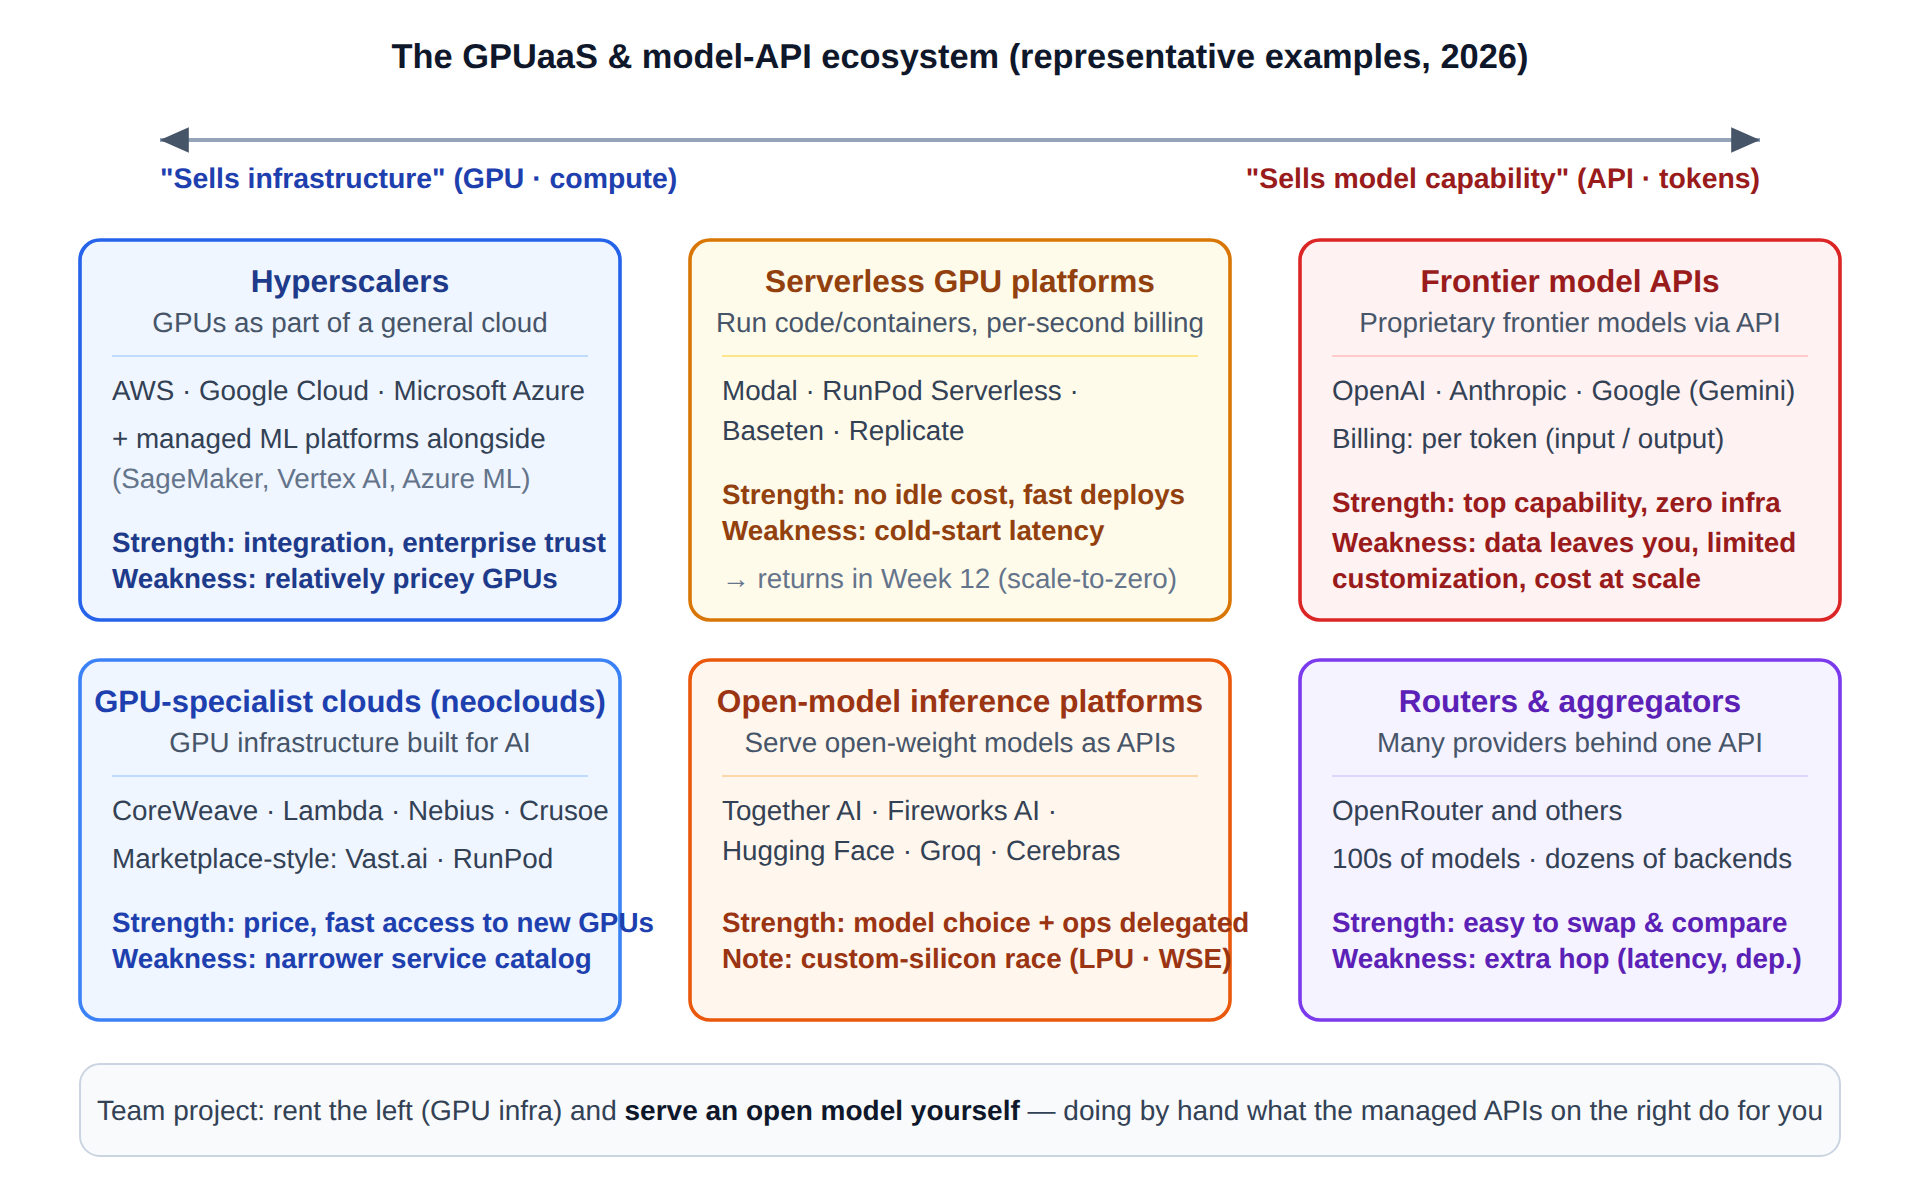
\includegraphics{figures/fig1-5_ecosystem.png}}\\[3pt]
  \figcaption{그림 1-5  GPUaaS와 모델 API 생태계. 왼쪽은 계산 자원을, 오른쪽은 역량을 판매한다. 회사 이름은 2026년의 예시일 뿐이며 중요한 것은 군집의 경계다.}
\end{tbbfigure}

\textbf{하이퍼스케일러}(AWS, Google Cloud, Azure)는 범용 클라우드의 일부로 GPU를 판매하며 관리형 ML 플랫폼도 함께 제공한다. 운영 중인 다른 모든 서비스와 통합하기 쉽고 보안과 규정 준수가 성숙했다는 장점이 있지만, GPU 가격에는 프리미엄이 붙는다. 시장에서 \textit{네오클라우드}라 부르는 \textbf{GPU 전문 클라우드}는 AI 워크로드를 위해 특별히 구축한 클라우드다. CoreWeave, Lambda, Nebius, Crusoe가 대표적이다. 새 GPU를 빠르게 도입하고 공격적으로 가격을 책정한다. Vast.ai 같은 마켓플레이스형 사업자는 유휴 GPU를 중개한다. 공급 변동성을 감수한다면 가장 저렴하다.

\textbf{서버리스 GPU 플랫폼}(Modal, RunPod Serverless, Baseten, Replicate, ...)은 서버라는 개념 자체를 숨기고 코드나 컨테이너 호출 단위로 GPU를 빌려 준다. 요청이 실행되는 동안에만 과금하므로 트래픽이 급증하거나 적은 서비스에 매력적이지만, 1.3절에서 만난 콜드 스타트가 약점이다. \textbf{오픈 모델 추론 플랫폼}(Together AI, Fireworks AI, Hugging Face, ...)은 공개된 오픈 웨이트 모델을 API 뒤에서 서빙한다. 직접 서빙할 때의 모델 자유도와 API의 운영 편의성을 함께 제공하는 중간 지대다. 이 군집에서는 Groq (LPU), Cerebras (WSE) 같은 기업이 GPU가 아닌 맞춤형 실리콘으로 속도 경쟁을 벌인다. 마지막으로 \textbf{프런티어 모델 API}(OpenAI, Anthropic, Google)는 폐쇄형 최첨단 모델을 토큰 단위로 판매하며, \textbf{라우터/애그리게이터}(OpenRouter 등)는 앞의 모든 서비스를 단일 API 뒤에 묶는다.

최근 몇 년 사이 이 지형을 가장 크게 바꾼 흐름은 \textbf{오픈 웨이트 모델의 부상}이다. 가중치를 공개적으로 내려받을 수 있는 Llama, Qwen, DeepSeek, Mistral 계열의 품질이 폐쇄형 모델을 따라잡으면서 "좋은 모델을 내 인프라에서 서빙한다"는 선택이 현실이 되었다. 자체 서빙 수요가 늘면 지도 왼쪽의 GPU 인프라와 가운데의 서빙 기술도 함께 성장한다. 이 책이 가르치는 내용이 바로 그 서빙 기술이다.

\subsection*{AI 서비스 경제의 장치: 키, 계량(meters), 할당량}

어느 군집에서 구매하든 거래의 형태는 공통적이다. 이 책에서 결국 직접 만들게 될 것이므로 이름을 붙여 둘 가치가 있다. 모든 모델 API와 GPU 플랫폼은 \textbf{API 키}(신원: \textit{누가} 호출하는가)를 발급하고, \textbf{계량기}(과금: 토큰당, 초당, 요청당)를 돌리며, 사용자를 \textbf{할당량과 속도 제한}(보호: 등급별 분당 요청 또는 토큰 상한) 안에 둔다. 상한을 넘으면 HTTP \textbf{429 Too Many Requests}를 받는다. 서비스 장애나 코드 오류가 아니라, 사용자의 트래픽이 다른 테넌트(tenant)에 피해를 주지 않도록 공급자의 로드 밸런서가 의도한 대로 정중히 거절한 것이다. 무료 등급, 사용량 대시보드, 지출 알림, 단계별 가격은 모두 키, 계량기, 울타리로 이루어진 같은 세 부분 장치다.

이처럼 평범한 일을 왜 장황하게 강조할까? 이 장치가 곧 제품이기 때문이다. 모델은 요청에 답하지만, 키·계량·할당량 장치가 요청에 답하는 행위를 \textit{사업}으로 만든다. 다른 사람이 운영하는 GPU 서버군을 예산에 넣을 수 있는 비용 항목으로 바꾸는 방법이다. 그리고 이 책이 닫으려는 고리가 바로 여기에 있다. 직접 서빙하는 순간, 당신이 곧 제공자가 된다. 그러면 모든 조각이 이번엔 당신의 책임으로 되돌아온다. 키를 확인하고 한도를 강제하던 API 게이트웨이는 6주차, 토큰당 원가를 알려주던 계량은 12주차, 그리고 팀 프로젝트는 바로 이런 정문 뒤에 자신의 모델을 내걸어야 한다. 6주차가 되면, 당신은 이 계산대의 반대편에 서 있게 된다.

\subsection*{자체 구축 대 외부 도입: 모델 API와 자체 서빙}

실제로 생태계의 두 끝은 하나의 결정으로 모인다. \textbf{모델 API를 구매할 것인가, 오픈 모델을 직접 서빙할 것인가?} 표 1-4에 판단 기준을 모았다.

\begin{tbbtablewrap}
  \begin{tabular}{@{}>{\raggedright\arraybackslash}m{\dimexpr 0.1915\tbltextwidth-2\tabcolsep\relax} >{\raggedright\arraybackslash}m{\dimexpr 0.4043\tbltextwidth-2\tabcolsep\relax} >{\raggedright\arraybackslash}m{\dimexpr 0.4043\tbltextwidth-2\tabcolsep\relax}@{}}
  \arrayrulecolor{tbbnavy}\specialrule{1pt}{0pt}{0pt}
  \rowcolor{tbbtablehead}{\centering \bfseries\color{tbbnavy}기준} & {\centering \bfseries\color{tbbnavy}모델 API에 유리(외부 도입)} & {\centering \bfseries\color{tbbnavy}자체 서빙에 유리(자체 구축)} \\
  \arrayrulecolor{tbbnavy}\specialrule{0.7pt}{0pt}{2pt}
  {\textbf{규모 / 트래픽}} & {작거나 불확실함 — 사용한 만큼만 지불} & {크고 일정함 — GPU를 포화 상태로 유지 가능} \\
  \arrayrulecolor{tbbtableborder}\hline
  {\textbf{데이터 / 규제}} & {데이터의 경계 외부 반출에 제약 없음} & {민감한 데이터, 온프레미스 또는 데이터 주권 요구 사항} \\
  \arrayrulecolor{tbbtableborder}\hline
  {\textbf{맞춤화}} & {범용 역량으로 충분함} & {미세 조정 모델, 특수 도메인, 출력 완전 제어} \\
  \arrayrulecolor{tbbtableborder}\hline
  {\textbf{지연 시간 제어}} & {공급자 SLA로 충분함} & {꼬리 지연 시간, 배칭, 하드웨어를 직접 조정해야 함} \\
  \arrayrulecolor{tbbtableborder}\hline
  {\textbf{팀 역량}} & {가용한 인프라 엔지니어가 없음} & {이 책으로 공부한 엔지니어가 있음} \\
  \arrayrulecolor{tbbtableborder}\hline
  {\textbf{최고 역량}} & {프런티어급 역량이 반드시 필요함} & {작업에 오픈 모델 품질로 충분함} \\
  \arrayrulecolor{tbbnavy}\specialrule{1pt}{2pt}{0pt}
  \end{tabular}\par
  \figcaption{표 1-4  모델 API와 자체 서빙의 선택 기준}
\end{tbbtablewrap}

비용 축은 빠른 어림 계산으로 살펴볼 수 있다. 아래 숫자는 \textbf{가상 값}이다. 소형 오픈 모델로 하루 토큰 2,000만 개를 생성하는 서비스를 가정하자. 토큰 100만 개당 \$0.5인 API를 쓰면 하루 \$10, 한 달에 약 \textbf{\$300}다. 같은 부하를 시간당 \$0.8인 L4 GPU 한 대로 직접 서빙하면서 상시 실행하면 한 달 약 \textbf{\$580}다. \textbf{이 규모에서는 API가 더 저렴하다.} 이제 트래픽이 20배 증가한다고 하자. API 청구액은 선형으로 늘어 \$6,000가 되지만, 자체 서빙 클러스터는 GPU 몇 대만 더 추가하면 따라갈 수 있다. 배칭이 처리량을 초선형으로 높이기 때문이다(10주 차). 중간 어딘가에서 두 곡선이 교차한다. 손익분기점을 제대로 찾으려면 GPU 사용률, 최적화 수준, 운영 인원까지 고려해야 한다. 팀 프로젝트의 "월간 운영 비용 추정"이 요구하는 작업이 바로 이것이다.

마지막으로 강조할 점은 이것이 양자택일이 아니라는 사실이다. 실제 조직은 흔히 \textbf{하이브리드 전략}을 쓴다. 프런티어 API로 프로토타입을 만들고 검증한 뒤, 성능이 입증되고 트래픽이 많은 핵심 부분을 자체 서빙 오픈 모델로 옮긴다. 어느 쪽을 선택하든 이 절의 목표는 \textbf{무엇을 포기하고 무엇을 얻는지 아는 상태에서} 선택하는 것이다.

\begin{calloutbox}{tbbpurple}{tbbpurplefill}
{\normalsize\bfseries\color{tbbpurple}생각해 보기}\par\vspace{3pt}
\begin{tbbitemize}
  \item 병원에서 임상 기록을 요약하는 AI를 도입하려 한다. 표 1-4의 기준을 적용해 보자. 어느 기준이 결정적인 장애물인가?
  \item 어림 계산 예시에서 자체 서빙 GPU의 사용률이 30\%에 불과해 하루 대부분을 유휴 상태로 보낸다고 하자. 실제 토큰당 비용은 어떻게 되는가? 사용률을 높이는 방법에는 무엇이 있는가? (12주 차 예고.)
  \item 자체 서비스의 트래픽이 급증한 동안 모델 API에서 429를 받았다. 이 역설을 추적해 보자. 공급자의 키·계량·할당량 장치 중 어느 부분이 \textit{공급자의} p99를 지키는 대가로 \textit{자체 서비스의} p99를 희생시켰는가? 공급자 서비스에 의존하는 동안 자체 서비스가 약속할 수 있는 SLO에 관해 무엇을 알려 주는가?
\end{tbbitemize}
\end{calloutbox}

\section{이 책의 로드맵과 학습 방법}

이 장에서 그린 큰 그림이 앞으로 15주 동안 어떻게 펼쳐지는지 살펴보자. 그림 1-6은 전체 로드맵이다.

\begin{tbbfigure}
  \adjustbox{max width=0.94\linewidth,max totalheight=0.46\textheight}{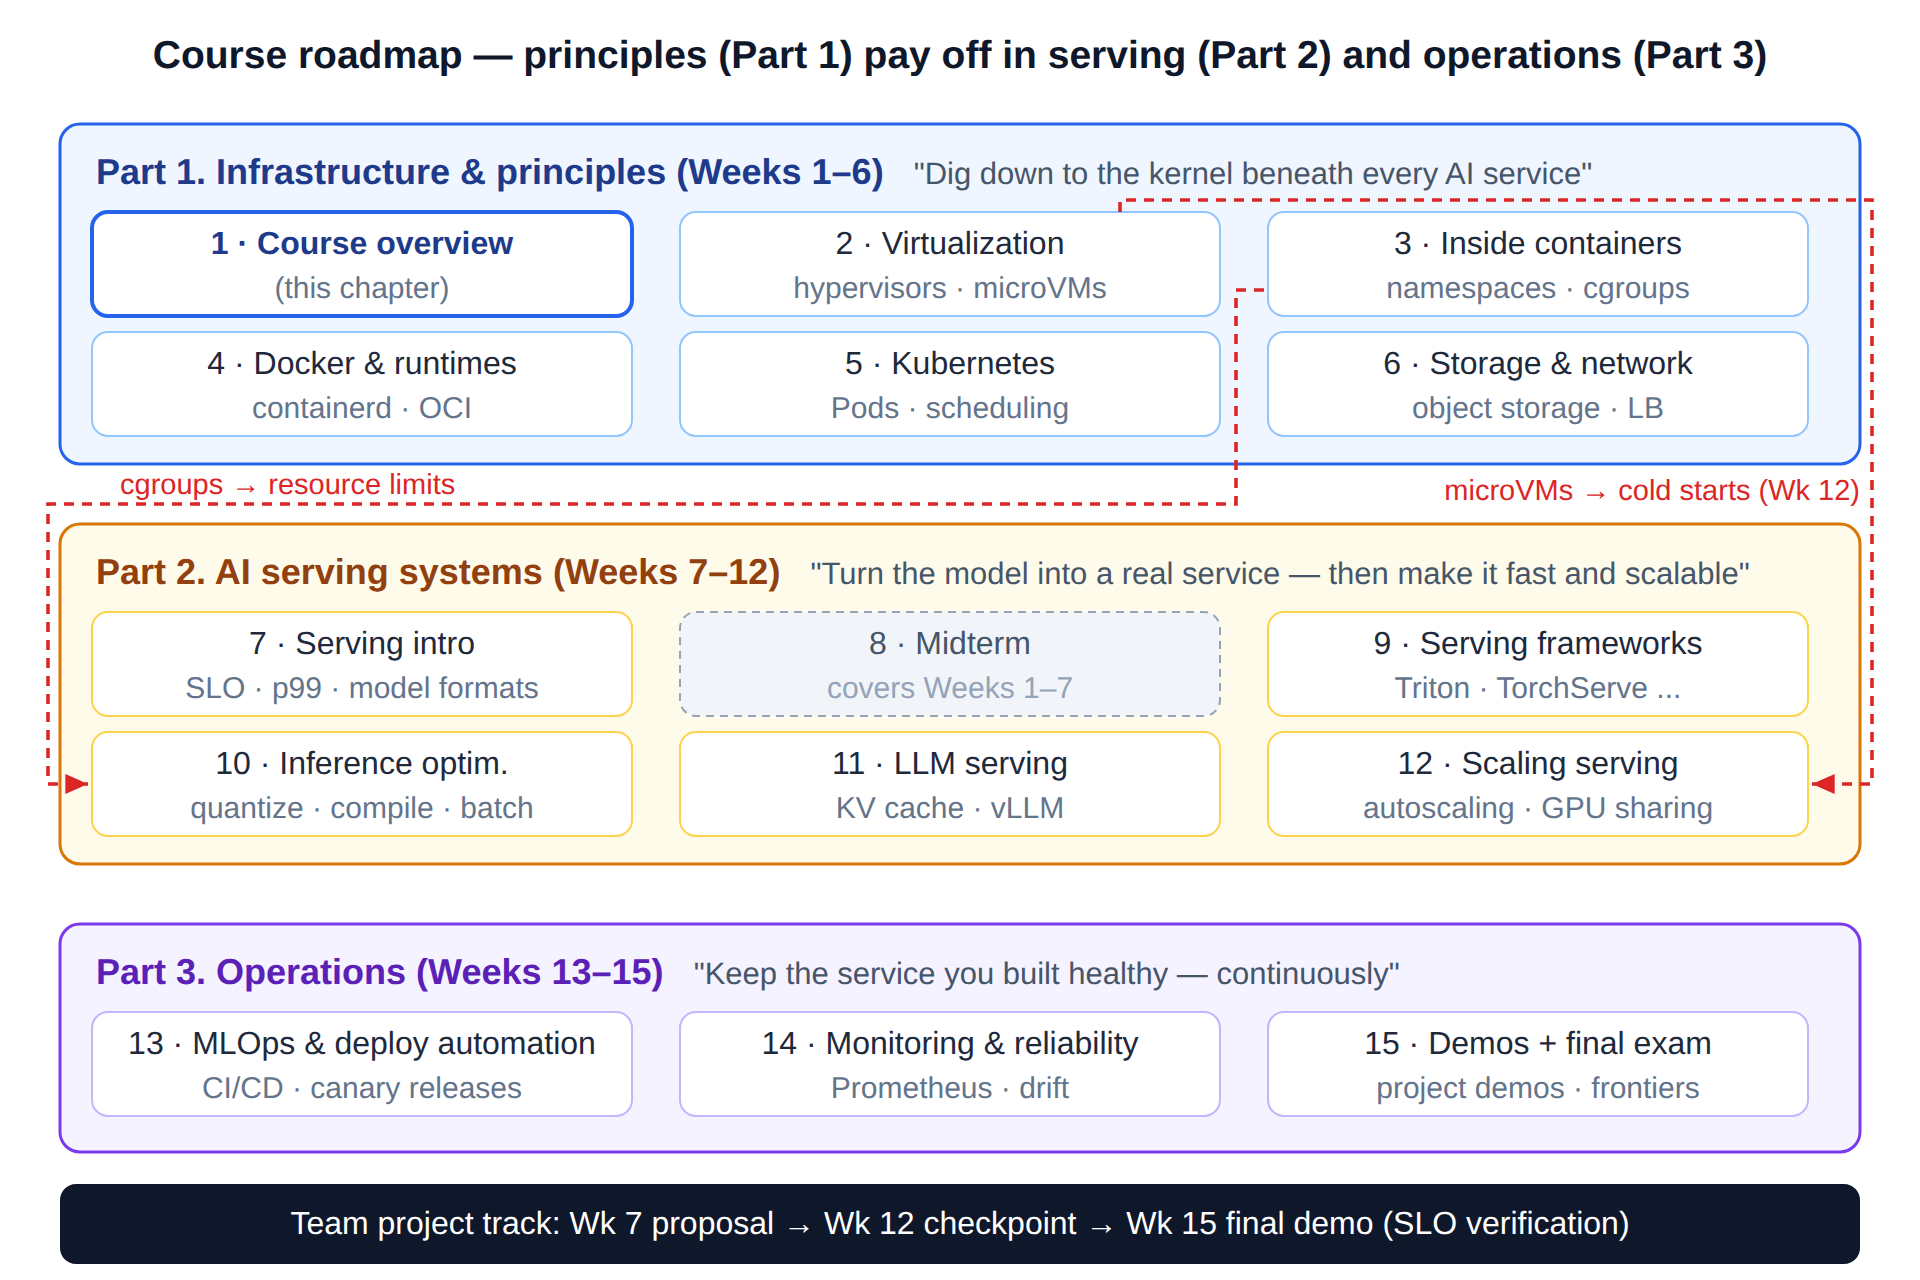
\includegraphics{figures/fig1-6_roadmap.png}}\\[3pt]
  \figcaption{그림 1-6  15주 로드맵. 빨간 점선은 제1부의 원리가 뒤의 주제에서 다시 호출되는 대표적인 경로를 표시한다.}
\end{tbbfigure}

\textbf{제1부(1\textasciitilde{}6주 차)}는 모든 AI 서비스가 서 있는 지반 아래의 커널까지 파고든다. 가상화(virtualization)가 CPU 명령어 수준에서 작동하는 방식(2주 차), 실제로 컨테이너를 구성하는 커널 기능(3주 차), Docker와 Kubernetes가 그 기능을 패키징하는 방식(4\textasciitilde{}5주 차), 모델 파일과 트래픽을 운반하는 스토리지와 네트워크의 모습(6주 차)을 배운다. \textbf{제2부(7\textasciitilde{}12주 차)}는 그 지반 위에 서빙 시스템을 구축한다. SLO와 p99라는 서빙 성능 언어(7주 차), 프레임워크로 실제 모델을 서빙하고 부하 테스트하기(9주 차), 양자화·컴파일·배칭으로 속도 높이기(10주 차), LLM 서빙의 독특한 세계(11주 차), 스케일링과 비용(12주 차)을 다룬다. \textbf{제3부(13\textasciitilde{}15주 차)}는 운영이다. 배포 자동화(13주 차), 모니터링과 신뢰성(14주 차), 팀 프로젝트 마무리(15주 차)로 이어진다.

로드맵이 강조하는 것은 빨간 점선, 즉 \textbf{콜백 구조}다. 이 책 전반부는 후반부를 예고하며, 의도적으로 되풀이되는 기념물을 여럿 만나게 된다. 나중에 다시 등장할 때 반갑게 알아볼 수 있도록 일부를 미리 소개한다.

\begin{tbbitemize}
  \item \textbf{숫자 137} — 이 장에서 수수께끼 같은 종료 코드로 처음 만나고, 3주 차에는 자기 프로세스에 직접 일으킨다(커널의 OOM 킬러다. 128 + SIGKILL의 9). 5주 차에는 Kubernetes가 이를 강제하며, 이후 내리는 모든 메모리 용량 결정에 따라붙는다.
  \item \textbf{수수께끼 같은 부모 프로세스 PID 41288} — 3주 차의 첫 번째 기록에서 컨테이너를 시작할 때 설명 없이 등장하고, 4주 차에 마침내 심문을 거쳐 정체가 밝혀진다. (미리 밝히지는 않겠다.)
  \item \textbf{1956년의 화물 컨테이너} — 4주 차는 강철 상자 하나가 화물 운송 비용을 \textasciitilde{}37× 줄인 이야기와 Docker 이미지가 소프트웨어에 같은 묘수를 적용한 이유로 시작한다. 이후에는 "컨테이너"라는 단어가 전과 달리 보일 것이다.
  \item \textbf{2주 차의 Firecracker microVM}(밀리초 만에 부팅되는 VM)은 12주 차의 \textbf{GPU 콜드 스타트}에서 돌아온다. "서버리스 GPU에서 첫 요청이 왜 느린가?"에 답하려면 머신이 부팅된다는 것이 물리적으로 무엇을 뜻하는지 알아야 한다.
  \item \textbf{3주 차에 직접 작성하는 cgroup 파일}(\code{memory.max}, \code{cpu.max})은 5주 차에 Kubernetes 자원 요청량/한도가 도달하는 바로 그곳이다. 하나의 메커니즘이 두 인터페이스를 쓴 것이며, 이 장의 밀도와 비용 절충에 대한 직접적인 답이다.
  \item \textbf{2주 차의 GPU 가상화}(PCIe 패스스루, vGPU, MIG)는 4주 차에서 커널 자체가 GPU 시간을 중재하지 못하는 이유를 설명한 뒤, 12주 차에 여러 서비스가 비싼 GPU 하나를 나누는 \textbf{GPU 공유} 전략으로 다시 등장한다.
\end{tbbitemize}

\subsection*{팀 프로젝트: 이 책의 종합 시험}

성적에서 가장 큰 비중(30\%)을 차지하는 팀 프로젝트의 과제는 한 문장으로 정리된다. \textbf{"오픈 소스 AI 모델을 선택해 클라우드에 배포하고, 목표 SLO를 충족함을 부하 테스트로 입증하라."} Kubernetes 기반 컨테이너 서빙, 부하 상황에서 SLO를 검증하는 오토스케일링, 모니터링 대시보드, 최적화 전후 비교, 월간 운영 비용 추정까지 이 장에서 둘러본 모든 주제가 프로젝트 하나에 들어간다. 제안서는 7주 차, 중간 점검은 12주 차, 최종 시연은 15주 차에 진행한다. 이번 주에는 팀을 구성하기만 하면 된다. 매주 배우는 내용을 차례로 조립하도록 설계한 프로젝트이므로 지금부터 겁먹을 이유는 없다.

\begin{tbbtablewrap}
  \begin{tabular}{@{}>{\raggedright\arraybackslash}m{\dimexpr 0.2553\tbltextwidth-2\tabcolsep\relax} >{\raggedright\arraybackslash}m{\dimexpr 0.1489\tbltextwidth-2\tabcolsep\relax} >{\raggedright\arraybackslash}m{\dimexpr 0.5957\tbltextwidth-2\tabcolsep\relax}@{}}
  \arrayrulecolor{tbbnavy}\specialrule{1pt}{0pt}{0pt}
  \rowcolor{tbbtablehead}{\centering \bfseries\color{tbbnavy}평가 요소} & {\centering \bfseries\color{tbbnavy}비중} & {\centering \bfseries\color{tbbnavy}평가 범위} \\
  \arrayrulecolor{tbbnavy}\specialrule{0.7pt}{0pt}{2pt}
  {중간고사} & {\centering 20\%} & {1\textasciitilde{}7주 차: 클라우드 인프라, 가상화 원리, 서빙 기초} \\
  \arrayrulecolor{tbbtableborder}\hline
  {기말고사} & {\centering 20\%} & {9\textasciitilde{}14주 차: AI 서빙 시스템 구축, 최적화, 운영} \\
  \arrayrulecolor{tbbtableborder}\hline
  {실습 과제} & {\centering 25\%} & {주별 실습 산출물과 벤치마크 보고서(5\textasciitilde{}6회 제출)} \\
  \arrayrulecolor{tbbtableborder}\hline
  {팀 프로젝트} & {\centering 30\%} & {제안서 · 중간 점검 · 최종 시연, 요구 사항과 SLO 달성 여부 평가} \\
  \arrayrulecolor{tbbtableborder}\hline
  {출석} & {\centering 5\%} & {대학 규정에 따름} \\
  \arrayrulecolor{tbbnavy}\specialrule{1pt}{2pt}{0pt}
  \end{tabular}\par
  \figcaption{표 1-5  평가 방식 한눈에 보기}
\end{tbbtablewrap}

\subsection*{실습 환경과 이번 주에 할 일}

실습은 AWS Academy 또는 Google Cloud for Education의 교육용 크레딧으로 진행한다. 모든 실습은 파라미터 1–3 B 규모의 소형 모델에 양자화를 적용한다는 가정 아래 T4 GPU 한 대나 Colab 세션 하나에서 실행되도록 설계했다. GPU가 전혀 없다면 \code{llama.cpp}를 통한 CPU 추론 경로로 대체할 수 있다. Kubernetes 실습은 비용을 아끼기 위해 기본적으로 로컬 환경(minikube/kind)을 사용한다. 이번 주에 할 일은 두 가지다. \textbf{① 환경 준비}(Python과 Docker를 실행할 수 있는 개인 노트북, 클라우드 교육용 크레딧 신청), \textbf{② 팀 구성}이다. 자세한 내용은 별도의 실습 안내서에서 설명한다.

\subsection*{이 책에서 좋은 성과를 내는 법}

네 가지 학습 조언이 있다. 첫째, \textbf{지금 선수 지식을 점검하라.} 2\textasciitilde{}3주 차부터 커널 수준의 내용을 다루므로 프로세스, 가상 메모리, 시스템 호출이 희미하게 느껴진다면 이번 주에 운영체제 과목을 복습하는 것이 가장 수익률 높은 투자다. Python 숙련도는 이 책 전체에서 전제로 삼는다. 둘째, \textbf{실습을 구경만 하지 마라.} 이 책의 지식은 남이 하는 모습을 지켜본 눈이 아니라 직접 \code{unshare}를 실행하고 네임스페이스를 만든 손에 쌓인다. 셋째, \textbf{어두운 상자를 재현하라.} 이 책에 실린 모든 터미널 기록(사례 1-A와 1-B 등)은 직접 실행하거나 산술적으로 검증할 수 있다. 제2장부터는 대부분 2주 차 실습에서 직접 빌릴 VM에서 실행된다. 직접 입력하라. 재현한 기록은 지식이고, 읽기만 한 기록은 잡학이다. 넷째, \textbf{계속 "왜"라고 물어라.} 모든 도구 뒤에는 그 도구가 해결하려고 탄생한 문제가 있다. "Kubernetes를 배웠다"보다 "Kubernetes 같은 것이 왜 존재해야 했는지 이해한다"가 더 가치 있다. 이 책이 추구하는 바가 후자이며, 이 책의 모든 장이 그 주의 기술을 필요하게 만든 재난, 청구서, 이야기로 시작하는 이유이기도 하다.

\namedsection{요약}{열두 가지로 정리한 제1장}

\qitem{1}{\textbf{모델은 서비스가 아니다.} 정확도는 모델의 속성이지만 동시성, 지연 시간, 가용성, 비용, 배포, 관측 가능성은 시스템의 속성이다. 사례 A는 정확도 94\%인 상태에서 실패했고, ChatGPT 출시는 모델링이 아니라 서빙 사건이었다. 프로덕션 ML 시스템에서 ML 코드는 작은 부분(Hidden Technical Debt)에 불과하며, 이 책은 나머지 전부를 다룬다.}

\qitem{2}{\textbf{사례 A의 계산은 일반화할 수 있다.} 서빙 시스템에는 처리량 상한(레플리카당 1 ÷ 요청별 시간)이 있다. 상한을 넘는 수요는 대기열이 되고, 대기열은 꼬리 지연 시간이 되며, 서비스 앞단의 구성 요소는 지나치게 긴 대기를 오류로 바꾼다. 서비스가 실패하는 데 어떤 것도 "충돌"할 필요는 없다.}

\qitem{3}{\textbf{사례 B의 계산도 일반화할 수 있다.} 상시 실행 용량은 트래픽 유무와 관계없이 매시간 과금된다. 기록해야 할 계량 지표는 사용률이며, 서빙 비용의 정직한 단위는 월이 아니라 요청당 비용(또는 토큰당 비용)이다.}

\qitem{4}{AI 서비스 스택은 \textbf{개발 → 학습 → 서빙 → 운영의 피드백 고리}이며, 모든 단계가 클라우드 인프라에서 실행된다. 이 책은 학습된 모델을 넘겨받는 시점부터 시작해 서빙과 운영을 책임진다.}

\qitem{5}{사용자가 체감하는 지연 시간은 모델 실행 시간이 아니라 \textbf{요청 경로의 합}이다. 성능 분석은 "어느 구간이 병목인가?"를 묻는 일이다.}

\qitem{6}{학습 워크로드는 \textbf{유한한 배치 작업으로, 처리량 중심이고 예측 가능하며 재시작할 수 있다.} 추론 워크로드는 \textbf{상시 실행 서비스로, 꼬리 지연 시간(p95/p99) 중심이고 부하가 급증하며 장애가 사용자에게 즉시 피해를 준다.} 후반부의 모든 주제(배칭, 오토스케일링, 콜드 스타트, 카나리 배포, 모니터링)는 이 대비에서 나온다.}

\qitem{7}{\textbf{지연 시간·처리량·비용으로 이루어진 서빙 삼각형은 이 책의 나침반이다.} 어느 하나를 지불하면 나머지 둘을 살 수 있다. SLO는 삼각형 위에서 의도적으로 선택한 점이며, 모든 최적화 주장은 무엇을 지불하는지 밝혀야 한다. 배칭, 양자화, 오토스케일링 같은 기법은 삼각형을 없애는 것이 아니라 움직인다.}

\qitem{8}{같은 모델에서 추론은 학습보다 훨씬 적은 메모리가 필요하지만, 메모리 사용량은 \textbf{시간에 따라 뾰족하게 출렁인다}(기준선인 가중치 + 부하 급증에 비례하는 활성값). 따라서 "관측한 유휴 사용량 + 10\%"를 메모리 한도로 삼는 것은 안전 여유가 아니라 예정된 OOM 처형(exit 137, 3주 차의 메커니즘)이다.}

\qitem{9}{클라우드 서비스 모델은 \textbf{"얼마만큼 빌리는가"}의 스펙트럼이다. GPU VM (IaaS) → 관리형 K8s (CaaS) → 관리형 엔드포인트 → 서버리스 GPU → 모델 API (SaaS)로 이어진다. 오른쪽으로 갈수록 제어권을 편의성과 교환한다. 이 책은 원리를 배우기 위해 의도적으로 왼쪽에서 직접 구축한다.}

\qitem{10}{GPUaaS 생태계는 \textbf{하이퍼스케일러 / GPU 전문 클라우드(네오클라우드) / 마켓플레이스 / 서버리스 GPU / 오픈 모델 추론 플랫폼 / 프런티어 모델 API / 라우터}로 이루어진다. 회사 이름은 바뀌지만 군집 구조는 남는다. 어느 군집에서든 인스턴스 선택은 \textbf{결정적인 제약 차원}, 보통 FLOPs가 아니라 메모리를 따라야 한다.}

\qitem{11}{AI 경제의 배관은 \textbf{키, 계량기, 할당량}이다(429는 장애가 아니라 울타리다). 자체 서빙을 하면 공급자가 되어 세 가지 모두 다시 구축한다. 6주 차의 게이트웨이, 12주 차의 계량기, 7주 차의 그 뒤에 있는 SLO다.}

\qitem{12}{이 책의 구조는 \textbf{원리(1\textasciitilde{}6주 차) → 서빙(7\textasciitilde{}12주 차) → 운영(13\textasciitilde{}15주 차)}이며, exit 137, PID 41288, 1956년의 화물 컨테이너, Firecracker, 모든 Kubernetes 한도 아래에 있는 cgroup 파일이 전반부와 후반부를 의도적으로 연결한다.}

\namedsection{연습문제}{}

\subsection*{A. 객관식}

\qitem{1}{AI 서비스 스택의 순서로 옳은 것은?}

\begin{tbboptions}
  \item ① 학습 → 개발 → 운영 → 서빙        ② 개발 → 학습 → 서빙 → 운영
  \item ③ 개발 → 서빙 → 학습 → 운영        ④ 학습 → 서빙 → 개발 → 운영
\end{tbboptions}

\qitem{2}{추론(서빙) 워크로드를 올바르게 설명한 것은?  ㉠ 시작과 끝이 있는 유한한 작업이다  ㉡ 지연 시간이 핵심 성능 지표다  ㉢ 사용자 트래픽에 따라 부하가 변동한다  ㉣ 체크포인트에서 재시작할 수 있으므로 장애 비용이 작다}

\begin{tbboptions}
  \item ① ㉠, ㉡        ② ㉡, ㉢        ③ ㉠, ㉣        ④ ㉢, ㉣
\end{tbboptions}

\qitem{3}{"p99 지연 시간 500 ms"의 정확한 의미는?}

\begin{tbboptions}
  \item ① 평균 응답 시간이 500 ms다
  \item ② 가장 느린 요청에 500 ms가 걸렸다
  \item ③ 전체 요청의 99\%에 500 ms 안에 응답했다
  \item ④ 요청의 99\%가 500 ms보다 오래 걸렸다
\end{tbboptions}

\qitem{4}{한 팀이 컨테이너 이미지를 만들고 관리형 Kubernetes(EKS/GKE)에 모델 서버를 배포한다. 이 선택을 가장 잘 설명한 것은?}

\begin{tbboptions}
  \item ① SaaS를 사용하는 것이므로 인프라 지식이 필요 없다
  \item ② CaaS 수준의 선택이다. 클러스터 운영은 위임하지만 컨테이너와 배포 명세는 계속 팀이 담당한다
  \item ③ GPU VM 전체를 빌리는 IaaS이므로 팀이 OS를 패치해야 한다
  \item ④ 서버리스이므로 유휴 상태에는 요금이 전혀 부과되지 않는다
\end{tbboptions}

\qitem{5}{자체 서빙(자체 구축)보다 모델 API(외부 도입)가 가장 분명히 유리한 상황은?}

\begin{tbboptions}
  \item ① 환자 기록을 구내 밖으로 반출할 수 없는 병원 시스템
  \item ② GPU를 포화 상태로 유지할 수 있을 만큼 트래픽이 크고 일정한 서비스
  \item ③ 트래픽이 거의 없는 아이디어 검증 단계의 MVP
  \item ④ 미세 조정 모델의 출력 형식을 완전히 제어해야 하는 서비스
\end{tbboptions}

\qitem{6}{파라미터 70 B 규모의 모델을 FP16(파라미터당 2 bytes)으로 로드하려 한다. 가중치만 고려할 때 80 GB H100 한 대에 대한 올바른 메모리 추정과 판단은?}

\begin{tbboptions}
  \item ① ≈ 70 GB — 들어간다        ② ≈ 140 GB — 들어가지 않는다
  \item ③ ≈ 35 GB — 들어간다        ④ ≈ 280 GB — 들어가지 않는다
\end{tbboptions}

\qitem{7}{한 팀이 GPU 서비스에 공격적인 배칭을 적용하자 GPU당 처리량이 60\% 늘고 토큰당 비용이 35\% 줄었다. 서빙 삼각형에 따르면 가장 가능성 높은 대가는 무엇이며, 어디에서 먼저 나타나는가?}

\begin{tbboptions}
  \item ① 모델 정확도 — 검증 점수
  \item ② 꼬리 지연 시간 — 요청이 배치가 찰 때까지 기다리면서 p95/p99에 나타남
  \item ③ 가용성 — 더 잦은 충돌
  \item ④ 없음 — 배칭은 대가 없는 개선임
\end{tbboptions}

\qitem{8}{추론 서버가 유휴 상태에서 6.0 GB를 쓴다. "관측한 유휴 사용량 + 10\%" 규칙에 따라 메모리 한도를 6.6 GB로 설정했다. 앞으로 벌어질 일을 가장 잘 예측한 것은?}

\begin{tbboptions}
  \item ① 안전하다. 10\% 여유가 현실적인 모든 변동을 감당한다
  \item ② 모델을 더 큰 크기로 다시 학습할 때만 위험하다
  \item ③ 위험하다. 활성값 메모리는 동시 요청 수와 입력 길이에 비례하므로, 처음으로 실제 부하가 몰리면 6.6 GB를 넘어 서버가 죽을 수 있다(exit 137)
  \item ④ 커널은 프로세스를 죽이지 않고 메모리를 스로틀링하므로 안전하다
\end{tbboptions}

\subsection*{B. 단답형}

\qitem{1}{"p99 지연 시간 ≤ 500 ms, 가용성 ≥ 99.9\%"처럼 표현하며, "서비스가 스스로 설정하는 정량적 품질 목표"를 무엇이라 하는가?}

\qitem{2}{0으로 스케일링은 유휴 상태일 때 서비스의 인스턴스를 0개로 줄인다. 조용한 시간이 지난 뒤 첫 요청이 인스턴스 시작과 모델 로딩을 기다리느라 매우 느려지는 문제를 무엇이라 하는가?}

\qitem{3}{빈칸을 채워라. 학습 워크로드의 주요 성능 지표는 ( ㉠ )이며, 온라인 추론 워크로드의 주요 성능 지표는 ( ㉡ )이다.}

\qitem{4}{파라미터 13 B 규모 모델의 가중치는 FP16에서 GPU 메모리를 약 얼마나 차지하는가? (계산 과정을 제시하라.)}

\qitem{5}{코드가 모델 API에서 HTTP 429를 받았다. 어떤 메커니즘이 이를 만들었으며, 이것이 코드의 버그나 공급자 서비스의 장애가 아닌 이유를 한 문장으로 설명하라.}

\subsection*{C. 서술형}

\qitem{1}{신입 팀원이 말한다. "모델의 검증 정확도가 94\%이므로 내일 서비스로 출시하겠습니다." 동시성, 지연 시간, 가용성, 비용, 배포, 관측 가능성 중 최소 세 가지 관점에서 시연과 프로덕션 서비스 사이의 간극을 구체적인 예로 설명하라.}

\qitem{2}{학습 워크로드와 추론 워크로드의 차이 중 두 가지를 선택하고, 각각이 만들어 내는 인프라 요구 사항(예: 스케줄러와 로드 밸런서, 수직 확장과 수평 확장)에 명시적인 논리 사슬로 연결하라.}

\qitem{3}{초기 스타트업이 법률 문서 요약 서비스를 만든다. 고객은 법률 회사 다섯 곳이고, 문서에는 민감한 계약 세부 사항이 담겨 있으며, 내년에 도메인 미세 조정 모델을 만들 계획이다. 모델 API(외부 도입), 자체 서빙(자체 구축), 단계적 전략 중 무엇을 권하겠는가? 현재 단계와 성장 단계를 구분해 표 1-4의 기준으로 논증하라.}

\qitem{4}{당직 엔지니어가 되어 사례 1-A를 다시 실행해 보자. 레플리카 하나는 한 번에 요청 하나를 0.25 s에 처리하고, 게이트웨이 타임아웃은 20 s이며, 사용자 80명이 도착해 연결을 유지한다. (a) 처리량 상한, (b) 대략적인 중앙값 대기 시간, (c) 504가 발생하는지 계산하라. 그런 다음 서빙 삼각형의 서로 다른 꼭짓점을 공략하는 해결책 두 가지를 제안하고 각각 무엇을 지불하는지 밝혀라.}

\namedsection{정답 및 해설}{}

\subsection*{A. 객관식}

\qitem{1}{\textbf{②} 개발(데이터, 실험) → 학습(모델 생성) → 서빙(서비스로 제공) → 운영(건강하게 유지)이며, 운영에서 개발과 학습으로 돌아가는 피드백 경로가 이들을 순환 고리로 연결한다. (1.2절)}

\qitem{2}{\textbf{②} ㉡과 ㉢이 옳다. ㉠은 학습을 설명하며(추론은 끝없이 상시 실행되는 서비스다), ㉣도 마찬가지다. 서빙 장애는 현재 사용자를 즉시 해치므로 비용이 크다. (1.3절)}

\qitem{3}{\textbf{③} 요청을 빠른 순서에서 느린 순서로 정렬했을 때 p99는 99번째 백분위의 지연 시간이다. 평균(①)은 느린 꼬리를 감추므로 서빙에서는 백분위 지표를 사용한다. (1.3절)}

\qitem{4}{\textbf{②} 관리형 K8s에서는 클러스터(컨트롤 플레인) 운영을 공급자에게 위임하지만, 이미지·배포 명세·서빙 구성은 사용자가 계속 책임진다. CaaS 수준이다. ③은 IaaS, ④는 서버리스 GPU를 설명한다. (1.4절, 표 1-2)}

\qitem{5}{\textbf{③} 트래픽이 적고 불확실하면 사용량 기반 API가 거의 언제나 더 저렴하며 더 빨리 출시할 수 있다. ①은 데이터 규제, ②는 규모, ④는 맞춤화에 관한 논거로, 모두 자체 서빙에 유리하다. (1.5절, 표 1-4)}

\qitem{6}{\textbf{②} 70 B × 2 bytes = 140 GB로, H100 한 대의 80 GB를 초과한다. 양자화하거나(예: 4-bit이면 약 35 GB) 여러 GPU에 샤딩해야 한다. 이런 추정에서 서빙 하드웨어 선택이 시작된다. (1.5절)}

\qitem{7}{\textbf{②} 배칭은 요청을 다른 요청과 함께 처리할 때까지 기다리게 하여 처리량과 비용을 얻는다. 가장 운이 나쁜 요청은 배치가 가장 많이 찰 때까지 기다리므로 대기 시간은 꼬리에 먼저 나타난다. 삼각형의 규율을 기억하자. 60\%/35\%의 이득도 실재하고 대가도 실재하므로, 엔지니어의 주장에는 둘 다 들어가야 한다. (1.3절)}

\qitem{8}{\textbf{③} 유휴 메모리는 기준선(가중치 + 런타임)이다. 요청별 활성값 메모리는 동시성과 입력 크기에 따라 늘어나므로 부하가 몰리면 유휴 상태보다 훨씬 높게 치솟는다. 6.6 GB 한도는 조용한 하루 내내 버티다가 처음으로 부하가 몰릴 때 서버를 처형한다. OOM 킬러가 보낸 SIGKILL이며 종료 코드는 137이다. 이 메커니즘(cgroup \code{memory.max})은 3주 차의 주제다. (1.3절)}

\subsection*{B. 단답형}

\qitem{1}{\textbf{SLO}(Service Level Objective, 서비스 수준 목표)다. 7주 차에는 SLI 및 SLA와 함께 발전시킨다.}

\qitem{2}{\textbf{콜드 스타트}다. GPU 서빙에서는 인스턴스 부팅 + 컨테이너 이미지 가져오기 + 모델 가중치 로딩이 겹쳐 수십 초에서 몇 분에 이른다. 12주 차에는 2주 차의 Firecracker와 함께 해결책을 다룬다.}

\qitem{3}{㉠ \textbf{처리량}, ㉡ \textbf{지연 시간, 특히 꼬리 지연 시간(p95/p99)}이다.}

\qitem{4}{13 B × 2 bytes/parameter = \textbf{≈ 26 GB}다. 24 GB L4에는 FP16으로 로드할 수 없어 양자화가 필요하다는 함의까지 덧붙이면 만점이다.}

\qitem{5}{\textbf{속도 제한 / 할당량}이다. 공급자의 허용 제어가 다른 테넌트와 공급자 자신의 p99를 보호하기 위해 사용자 등급의 상한을 넘는 요청을 거절한다. 의도대로 작동한 울타리이며, 해결책은 백오프(backoff) 후 재시도, 상위 등급 사용, 또는 직접 같은 울타리를 구축하는 자체 서빙(6주 차)이다.}

\subsection*{C. 서술형(채점 기준)}

\qitem{1}{핵심 명제는 정확도가 시스템 품질을 전혀 보장하지 않는다는 것이다. 동시성(동시 요청, 대기열), 지연 시간(경로의 합, 꼬리), 가용성(자동 복구, 무중단), 비용(유휴 GPU), 배포(롤링 교체, 롤백), 관측 가능성(메트릭이 없으면 고장 사실조차 알 수 없음) 중 세 가지 이상을 각각 서비스 맥락의 예와 연결하면 만점이다. (1.1절)}

\qitem{2}{모범 답안 예시: ① "작업과 서비스" → 학습에는 배치 스케줄러와 작업 대기열이 필요하고, 서빙에는 로드 밸런서, 오케스트레이터, 자가 치유가 필요하다. ② "처리량과 지연 시간" → 학습은 큰 배치로 GPU를 포화시키지만, 배칭은 지연 시간을 늘리므로 서빙은 동적 배칭으로 절충해야 한다. 부하 패턴 → 오토스케일링, 장애 비용 → 레플리카와 카나리 배포, 통신 패턴 → 수직 확장과 수평 확장도 옳다. 차이를 단순히 나열하지 않고 인프라 결과에 \textit{연결했는지}가 채점의 핵심이다. (1.3절)}

\qitem{3}{유일한 정답은 없으며 논증을 평가한다. 좋은 논리는 다음과 같다. 민감한 데이터(규제)와 미세 조정 계획(맞춤화)은 자체 구축을 가리키지만, 고객 다섯 곳이라는 작은 규모는 외부 도입을 가리킨다. 따라서 단계적 전략을 쓴다. (a) 현재는 개인정보를 보호하는 계약 아래 API로 빠르게 검증한다. (b) 규제로 불가능하다면 소형 오픈 모델의 자체 서빙으로 시작한다. (c) 미세 조정/성장 단계에는 자체 서빙으로 확실히 전환한다. 표 1-4의 기준을 명시적으로 사용하고 손익분기점을 어느 정도 추론해야 한다. (1.5절)}

\qitem{4}{(a) 레플리카당 1 ÷ 0.25 s = \textbf{4 req/s}다. (b) \textasciitilde{}80개 연결이 유지되므로 중앙값 요청은 \textasciitilde{}40개 요청 뒤에 선다. 40 × 0.25 ≈ \textbf{10 s}다. (c) 가장 긴 대기열은 \textasciitilde{}79개이므로 79 × 0.25 ≈ 19.8 s다. 20 s 타임아웃 바로 아래이므로 \textbf{아직은 504가 거의 발생하지 않는다}. 다만 서비스 시간의 작은 변동이나 사용자 한 차례만 더 몰려도 꼬리가 절벽을 넘는다. 계산을 제시하고 어느 쪽이든 논증하면 만점이다. 해결책은 다음 중 두 가지를 제시하고 꼭짓점을 밝혀야 한다. 레플리카 추가(지연 시간과 처리량을 얻고 비용을 지불), GPU 배칭(처리량/비용을 얻고 꼬리 지연 시간을 지불), 동시성 제한과 빠른 부하 차단(허용된 요청의 지연 시간을 보호하고 처리량 형태의 가용성을 지불), 더 작거나 양자화된 모델로 요청을 빠르게 처리(삼각형을 이동하며 엔지니어링 시간과 경우에 따라 품질을 지불)다. (1.1절, 1.3절)}

\namedsection{더 읽을거리}{}

더 깊이 파고들고 싶은 독자를 위한 자료다. ◆는 과정 교재를, ▶는 특정 주차에 다시 만날 자료를 표시한다.

\begin{tbbitemize}
  \item ◆ \textbf{Chip Huyen, Designing Machine Learning Systems (O'Reilly, 2022)} — 주 교재다. 이 장과 관련해서는 제1장(큰 관점의 ML 시스템)과 제7장(모델 배포와 예측 서비스)을 먼저 읽는다. ML을 시스템 관점에서 보는 능력을 기르기에 가장 좋은 단 한 권이다.
  \item ◆ \textbf{Chip Huyen, AI Engineering (O'Reilly, 2025)} — 파운데이션 모델 시대에 맞게 그림을 갱신한 부 교재다. 제9장(추론 최적화)은 이 책의 10\textasciitilde{}11주 차와 짝을 이룬다.
  \item \textbf{D. Sculley et al., "Hidden Technical Debt in Machine Learning Systems," NeurIPS 2015} — 1.1절에서 인용한 "ML 코드는 작은 상자" 그림의 출처다. 10쪽 남짓이므로 이번 주에 원문을 읽어 보자.
  \item ▶ \textbf{A. Agache et al., "Firecracker: Lightweight Virtualization for Serverless Applications," NSDI 2020} — 2주 차 필독 자료다. AWS Lambda 아래의 microVM 설계이자 이 장에서 예고한 콜드 스타트 이야기의 기술적 뿌리다.
  \item ▶ \textbf{W. Kwon et al., "Efficient Memory Management for Large Language Model Serving with PagedAttention," SOSP 2023} — 11주 차 필독 자료다. 운영체제 페이징을 LLM 서빙으로 이식한 vLLM의 핵심 아이디어를 다룬다. 이 책의 정신에 이보다 더 잘 맞는 논문은 없다.
  \item ▶ \textbf{Liz Rice, "Containers from Scratch" (GOTO 2018, video)} — 3주 차 실습의 원전이다. 수십 줄의 Go 코드로 아무것도 없는 상태에서 컨테이너를 만드는 30분짜리 영상이다. 보고 나면 컨테이너를 둘러싼 신비감이 사라진다.
  \item ▶ \textbf{Google SRE, Site Reliability Engineering (O'Reilly, 2016), Chapter 4 "Service Level Objectives"} — 온라인에서 무료로 읽을 수 있으며, 이 장이 서빙 삼각형으로 예고한 SLO 규율을 정석적으로 다룬다. 이 용어 체계를 그대로 도입하는 7주 차 전에 읽는다.
  \item \textbf{[이번 주의 흥미로운 읽을거리] ChatGPT 출시 후 첫 100일을 다룬 당시 보도} — 예를 들어 1억 사용자 추정치를 보도한 Reuters의 2023년 2월 1일 기사와 OpenAI 상태 페이지의 과거 기록이 있다. 팬이 아니라 서빙 엔지니어의 눈으로 읽어 보자. 모든 일화가 사상 최대 규모로 대중 앞에서 이루어진 용량, 대기열, 비용 결정이다.
  \item \textbf{기술 문서} — Kubernetes Concepts 페이지(5주 차 전에 훑어본다), OCI Runtime Specification, Linux cgroups v2 커널 문서, vLLM · NVIDIA Triton · TensorRT 공식 문서가 있다. 소설이 아니라 사전처럼 활용하라.
  \item \textbf{생태계 관찰} — GPU 가격과 공급자 지형은 고정된 참고 자료가 따라잡기 어려울 만큼 빠르게 변한다. 중요한 것은 확인하는 습관이다. 클라우드 가격 페이지, 서빙 엔진 릴리스 노트, NSDI · OSDI · SOSP · MLSys의 서빙 논문은 주기적으로 관찰하기 좋은 지점이다.
\end{tbbitemize}

\vspace{5.0pt}

\begin{calloutbox}{tbbblue}{tbbbluefill}
{\normalsize\bfseries\color{tbbblue}다음 장 — 제2장: 가상화 원리와 클라우드 컴퓨팅}\par\vspace{3pt}
이 장에서는 "클라우드에서 GPU VM을 빌린다"고 자연스럽게 말했다. 다음 장은 작은 충격으로 끝나는 심문에서 시작한다. 엄밀히 말해 빌린 머신은 존재하지 않는다. 임대의 실제 의미를 열어 본다. 물리 서버 하나를 여러 "가상" 머신으로 나누는 방식(하이퍼바이저, Intel VT-x / AMD-V), Linux 자체가 클라우드의 하이퍼바이저가 된 과정(KVM/QEMU, virtio), 밀리초 만에 부팅되는 VM을 가능하게 하는 기술(Firecracker microVM), 실재하는 GPU를 가상의 컴퓨터 안에 넣는 방식(PCIe 패스스루, vGPU, MIG)을 배운다. 실습에서는 클라우드 계정을 만들고, 사례 1-B를 기억하며 가장 먼저 과금 알림을 설정한다. 그런 다음 첫 VM을 시작해 같은 추론 작업에서 CPU와 GPU의 속도를 겨룬다.
\end{calloutbox}
